\documentclass[a4paper,12pt]{report}

\usepackage[utf8x]{inputenc}
\usepackage[english]{babel}
\usepackage[T1]{fontenc}
\usepackage{lmodern}

\usepackage{amsmath}
\usepackage{amssymb}
\usepackage{geometry}
\usepackage{a4wide}
\usepackage{enumerate}
\usepackage{graphicx}
\usepackage{lastpage}
\usepackage{cite}
\usepackage[pdftex]{hyperref}
\usepackage{caption}
\usepackage{subcaption}

\linespread{1.2}

\usepackage{fancyhdr}
\pagestyle{fancy}
\fancyhead{}
\fancyfoot{}

\newcommand{\myname}{Axel Angel}
\newcommand{\mytitle}{Towards Distortion-Predictable Embedding of Neural Networks}
\newcommand{\mysubtitle}{Thesis}
\newcommand{\mydate}{\today}

\newcommand{\N}{\mathbb{N}}
\newcommand{\Z}{\mathbb{Z}}
\newcommand{\Q}{\mathbb{Q}}
\newcommand{\R}{\mathbb{R}}
\newcommand{\C}{\mathbb{C}}

\lhead{\myname}
\rhead{\mytitle{} - \mysubtitle{}}
\chead{}
\rfoot{Page \thepage\ of \pageref{LastPage}}
\lfoot{\mydate}

\makeatletter
\AtBeginDocument{
  \hypersetup{
    pdfauthor = {\myname},
    pdftitle = {\mytitle},
    pdfsubject = {\mysubtitle},
  }
}
\makeatother

\newcommand{\eg}{e.g.}
\setkeys{Gin}{width=0.75\textwidth}

%\renewcommand{\includegraphics}[2][0]{\relax} % FIXME: figures disabled

\begin{document}
%First page (make guard, epfl logo, prof names, title, etc)
\begin{titlepage}
\begin{center}
    \vspace*{0.5cm}

    \line(1,0){400}
    \vspace{0.5cm}

    {\bf \Large Towards Distortion-Predictable Embedding}

    \vspace{0.5cm}

    {\bf \Large of Neural Networks}

    \vspace{0.5cm}
    \line(1,0){400}

    \vspace{1.5cm}

    {\bf \myname}

    Master of Computer Science

    \vspace{1.6cm}

    Supervised by

    {\bf Prof. Pascal Fua}

    {\bf Dr. Sironi Amos}

    \vspace{0.8cm}

    Computer Vision Laboratory (CVLAB)

    École Polytechnique Fédérale de Lausanne (EPFL)

    \vspace{3cm}

    \today

    \vfill

    \includegraphics[width=0.3\textwidth]{thesis_figures/epfl_logo.png}


    \end{center}
\end{titlepage}

\newpage
\thispagestyle{empty}
\vfill
\begin{center}
    Page intentionally left blank.
\end{center}

\cleardoublepage
\begin{abstract}
    Current research in Computer Vision has shown that {\em Convolutional Neural Networks} (CNN) give state-of-the-art performance in many classification tasks and Computer Vision problems\cite{mnist_web}\cite{krizhevsky2012imagenet}\cite{rowley1998neural}\cite{prechelt1994proben1}.
    The embedding of CNN, which is the internal representation produced by the last layer, can indirectly learn topological and relational properties.
    Moreover, by using a suitable loss function, CNN models can learn invariance to a wide range of non-linear distortions such as rotation, viewpoint angle or lighting condition.
    In this work, we provide insights about CNN embeddings and propose a new loss function, derived from the contrastive loss, that creates models with more predicable mapping and also quantifies distortions.
    Usual distortion-dependant methods would require to feed-forward inputs under every distortions because no simple relation would exist between their features.
    Our contribution makes a step towards embeddings where features of distorted inputs are related and can be derived from each others by their intensity.
    We also introduce a simple method to compare quantitatively embeddings of models which are used for dimensionality reduction. %whose purpose is to capture topological structures of particular distortions.
\end{abstract}

% ==============================================================================
\tableofcontents


% ==============================================================================
\chapter{Introduction}

Nowadays Computer Science has become predominant in many fields of science for data storage, data analysis, and many more.
The amount of data is increasing every day and computers are made faster to explore more complex problems.
There is an enormous flow of information in terms of quantity and dimensions: sound, images and videos are common.
Many area of science need methods to extract specific information out of these growing data.
This is usually done through analysis, visualization, or even both combined.

Computer Vision (CV) is a field addressing the problem of analyzing visual multimedias by automatic processing means.
To name a few examples: image classification and pattern recognition.
Many state-of-the-art solutions are combining the advance of Machine Learning to find models statistically instead of designing algorithms by hand which usually requires expert knowledge of the domain.
For example {\em Convolutional Neural Networks} (CNN), which is a ``visual'' variant of {\em Neural Network}s (NN), are now widely used for Computer Vision with great success\cite{krizhevsky2012imagenet}\cite{rowley1998neural}\cite{prechelt1994proben1}.
They are trained in a supervised way to perform a systematic processing task like for instance image classification (\eg: a handwritten digit) into a number of fixed categories (\eg: 0 through 9).
The {\em Features} are the internal representation of the input inside NN that they optimize during training to give better results.
In common classification tasks, the features are meant to lie in a low dimensional space and should be more compact than the input.
Therefore, these NN can be seen as two embedded parts: a dimensionality reducer that extracts important informations and a classifier that takes a decision based on these features.
Most practical applications will have to deal with some form of image distortions in their data: shearing, noise, camera viewpoint, lighting condition, to name a few.
In the case of classification, distortions can require putting extra efforts to train a ``resistant'' model which still classifies correctly its input in the presence of such deformations.
Most implementations decide to just kill the distortion signal with data-augmentation (which assigns the original label on distorted samples) because they do not need this information eventually.
However there are practical use cases that would benefit from having a quantified and predictable signal of the distortions coded into their features.

Our first step towards our research is to better understand NN embeddings and see if we can use conventional tools to extract distortion features reliably.
Moreover, visual inspection of the feature space using a human-friendly representation can help to gain insights and improve our models.
One way to analyze the features is to apply methods that project highly-dimensional points into lower space such as dimensionality reduction.
Many differences characterize dimensionality reduction methods such as: properties, flexibility and final goals.
We will do a brief overview of them: PCA, LLE, Isomap and more recently SNE.
However many of them lack in flexibility by representing only linearity while many of the rest still cannot preserve hierarchical structures accurately\cite{t-SNE}.
Researches have shown that t-SNE, a variant of SNE, has greatly improved on this regard: it is capable of keeping global clusters and fine-grained coherence inside them.
Moreover it was used multiple times successfully to visualize the feature space of NN\cite{donahue2013decaf}\cite{yu2014visualizing}.

Nonetheless, t-SNE is not a perfect solution and it has its own drawbacks as well.
First, like unsupervised methods it cannot be controlled directly because t-SNE is only given unlabelled points.
Therefore, as we will show later, the resulting embedding can have an unexpected shape unfit for the target application.
Secondly, this method works directly on the representations of the points without creating a mapping that computes the relation between input and output.
Thus it is impossible to compute the representation of points that were not part of the optimization process at the beginning.
It would be necessary to recompute the whole representation from scratch with these new points which is not fast to start with.
In this work, we show how we tried to combine CNN and t-SNE to produce an embedding that quantifies distortions in a predictable way.
However the resulting embeddings are unexpectedly messy: distortions are the primary factor of clusters, digit classes are not well separated and we faced problems to scale t-SNE to larger datasets.
We could have improved t-SNE to leverage external prior-informations such as labels but the faced shortcomings were quite important.

An alternative dimensionality reduction method consists of using the NN to directly compute an embedding similar to t-SNE but trained in a supervised manner.
The network is used to learn a mapping from the image space to a lower embedding which does not have the previous shortcomings and can satisfy the properties we described above.
As NN have the capacity to represent any non-linear continuous functions\cite{csaji2001approximation}, it is suitable to compute a very powerful dimensionality reduction method, hopefully very similar to t-SNE.

To achieve this goal, {\em Reduction by Learning an Invariant Mapping} ({\em DrLIM}) has combined concepts similar to the ones employed in t-SNE but expressed in an equivalent adapted formulation for NN.
%By using this new formulation, we can progress on the research of dimensionality reduction methods employing neural networks.
The key elements in their paper are: the contrastive loss function with the Siamese network architecture for training and a pairing strategy directly describing the embedding.
The current formulation allows to express a one-dimensional relation between two pair of images based on the similarity: similar pairs of images should be close together whereas dissimilar pairs should be further.
In this work, we extend DrLIM by introducing a generalized loss function.
Our extension allows to express a N-dimensional similarity relation between pairs of images and each similarity is expressed in the embedding only by a number of dimensions of choice.

Therefore, it becomes possible to control more finely the embedding through our extension.
We will follow the experiments made on DrLIM and train our own model on a data-augmentation of the MNIST dataset\cite{lecun1998mnist} with translations or rotations then we do the same on the NORB dataset\cite{lecun2004learning}.
The resulting embeddings are studied in details with multiple comparisons to DrLIM.
We find that we can embed distortion information in one extra dimension while reasonably preserving the characteristics of DrLIM on MNIST.
We also find that our solution can represent the DrLIM's coherent and cyclic space of the camera viewpoint on NORB.
The successful application on these two datasets demonstrate the effectiveness of our method.

\section{Thesis Outline}
% FIXME: list chapters with their summarzied content
In Chapter~\ref{chap:related}, we introduce the previous papers that are related to our current work.
We take a look at the prior arts in dimensionality reduction and the advance of Computer Vision with NN.
Then we will introduce our most important reference paper introducing DrLIM models.

In Chapter~\ref{chap:neural_network}, we recap the background knowledge necessary to understand the networks used in our experiments.
We also discuss the general architecture of NN, their similarity with CNN and some important definitions.

This is followed by Chapter~\ref{chap:dim_red} where the standard dimensionality reduction methods are reviewed in more details.
We explain the major advantages and drawbacks of one particular method, t-SNE, compared to other methods.
Later in the chapter, we provide the basic theoretical knowledge behind t-SNE optimisation problem.
Next we talk about the necessary tools to achieve dimensionality reduction with NN and how we extend the contrastive loss to N-dimensional similarity.

In Chapter~\ref{chap:results}, we describe our experiment environment in terms of technical choices (software, network architecture and datasets).
This chapter also includes all our practical results, our hypothesises and also our early conclusions.

And finally in Chapter~\ref{chap:conclusion}, we give our final conclusions about our results and the future works that can start from our contributions.


% ==============================================================================
\chapter{Related Work}
\label{chap:related}
% explain each paper, group them and discuss result adv/drawbacks

More than 20 years ago, researchers discovered that NN is a highly flexible model architecture to solve many classification problems.
Most of today models are using {\em Convolutional Neural Networks} (CNN) which are a powerful and specialized variant for visual tasks like MNIST \cite{mnist_web} and ImageNet \cite{krizhevsky2012imagenet}, face detection as well \cite{rowley1998neural} and many more \cite{prechelt1994proben1}.
This architecture is more efficient for Computer Vision problems, partly because the convolutions share their weights in the first layers to extract spatial cues.

Current researches is mainly focused on advancing into more complex classification problems using Deep Learning.
This field suggests improving the current results by deepening the architecture in terms of number of layers to express more abstract and higher-level concepts.
Unfortunately, more layers require more computations than before due to the increase of parameters but researchers started to overcome this challenge.
Ways to speed up the training and the classification appeared and were greatly beneficial for the development of this field in recent years\cite{ciresan2011flexible}\cite{schmidhuber2015deep}\cite{nasse2009face}.
The use of GPUs parallelism and cloud computing allowed scaling up to much deeper architecture (with many more parameters) than before\cite{coates2013deep}.
%paper: Flexible, high performance convolutional neural networks for image classification
Both researchers and professional programmers built various frameworks to train and to use NN with many different goals such as: performance, accessibility or composability.
The most popular are: Theano\cite{bastien2012theano}, Caffe\cite{jia2014caffe}, Torch7\cite{collobert2011torch7}, Pylearn2\cite{goodfellow2013pylearn2}.
We decided to leverage the efficiency and modularity proposed by Caffe for several reasons described later.
%deeper architectures improves accuracy on more complex tasks, people found optimisations to make them fast.

Even though CNN models are now widely used in Computer Vision with great success thanks to these frameworks, current research exposed our ignorance of these networks behaviors.
Some papers work on reliable ways to fool networks using adverserial attacks which exploits their unintuitive properties\cite{szegedy2013intriguing}.
Most publications do not try to formally justify their good results because of the non-linear and complex relations between units. % FIXME: citation needed?
%paper: Intriguing properties of neural networks
Moreover, this problem is stressed by distortions present in the inputs as well.
%Moreover the input-output relation, when inputs are kept distorted on purpose, is usually either killing the signal (invariance) or not in a predictable manner (controlled preservation).
It is not possible to directly look at the high-dimensional embedding, because we cannot easily plot nor interpret so many dimensions.
The manifestation of this relation can be looked visually using methods to produce an alternative human-friendly representation.

% moved from dim red chapter
Dimensionality reduction methods is a popular tool in such a case\cite{dai2014document}\cite{taylor2011learning} and several methods exist that are specialized for visualization.
Standard methods, like PCA and MDS\cite{cox2000multidimensional}, are used for reducing dimensions usually as a preprocessing step and they are limited to linearity in the data.
Their primary characteristic is to maximize the variance of the original data which is important for reconstruction but not necessarily for visualization.
Other non-linear dimensionality reduction methods, for instance: Isomap\cite{tenenbaum2000global}, LLE\cite{roweis2000nonlinear} and SNE\cite{SNE}, solve an optimisation problem with a loss function which improve their flexibility for purposes like visualization and preserve local structure/cluster.
However, recent papers show that SNE has better potential to keep global clusters and local details at the same time unlike the other previously cited methods\cite{SNE}.
%paper: Stochastic Neighbor Embedding

SNE has introduced a better maximization problem to preserve point neighborhood and general clusters with an important emphasis on distances\cite{SNE}.
%Kullback-leibler divergence.
However it suffers from ``center-crowdedness'' and faces difficulties in optimisation\cite{t-SNE}.
That's why papers are using t-SNE, a variant of SNE, to reduce CNN embeddings into a 2D human-friendly manifold. % FIXME: more cite?
This method exhibits an easier optimisation formulation and it preserve more structures at diverse scales.
More convincing examples were created with t-SNE directly from raw popular datasets\cite{van2009new} like MNIST\cite{t-SNE}.
A more recent work proposed an alternative method, called Barnes-Hut SNE, that approximates t-SNE with a much faster algorithm but we do not use it in our work.

Many more details in CNN embeddings appears by using t-SNE such as: how samples are grouped depending on multiple factors: essentially based on similarity of the digits (strokes, thickness and shapes) and natural variance (rotation).
%Although it is unintuitive, this can be seen by inspecting the embedding.
%we can add constraints against distortions directly over the embedding, to cluster them the way we meant.
Many papers use dimensionality reduction to create a human viewable representation of the output embedding \cite{donahue2013decaf}\cite{yu2014visualizing}\cite{yaotiny}.
Only a few papers actually try to formalize the input-output relations\cite{goodfellow2009measuring}.
Some papers proposes to learn transformation-invariant embeddings, by means of modelling distortions directly into their models\cite{gens2014deep} or using data-augmentation\cite{hadsell2006dimensionality}.
%paper: Encoded Invariance in Convolutional Neural Networks
%paper: Deep Symmetry Networks
%proposes an alternative network, symmetry networks, to extend invariance beyond translation by using feature map over arbitrary symmetry groups by use of kernel-based interpolation.
%paper: Dimensionality Reduction by Learning an Invariant Mapping

The latter proposes to create a dimensionality reducing mapping, called {\em Reduction by Learning an Invariant Mapping} ({\em DrLIM}), by training a CNN using a new loss function based on energy models, called the {\em contrastive loss}.
This paper will be mentioned in this work as the {\em reference paper} or DrLIM's paper.
Their results using on the MINST dataset\cite{lecun1998mnist} shows that CNN can learn a mapping that distinguish labels, and group alike digits even when they are translated artificially.
They experimented with the NORB dataset\cite{lecun2004learning} as well with intriguing results: each sample is mapped on a 3D cylinder whose axes quantify the orientation in 2D and the azimuth angle in 1D.
The network was successfully trained to ignore lighting conditions, which is a strongly non-linear distortion.
They use the Siamese training architecture to present image pairs which are optimized to be close if similar or far otherwise\cite{bromley1993signature}\cite{chopra2005learning}.
There are several advantages of such a method: the cost penalty is very low and present only during training, the usage of standard CNN allows more freedom for experimenting with different architectures and the proposed loss function is effective while simple.

%Moreover the input-output relation, when inputs are kept distorted on purpose, is usually either killing the signal (invariance) or not in a predictable manner (controlled preservation).
However the input-output relations of distorted images is usually damped instead of being quantified in a predictable way.
We think that the distortion information should be kept because they are valuable later on.
Besides, the reference paper provides subjective comments of the embedding coherence (description and figure) but they do not offer nor propose a formal way to measure and compare its quality objectively.
We used this paper as our primary reference for experiments to continue improving their ideas in this work.

In this work, we will present a practical solution towards predictable embedding with respect to distortion and offer a qualitative measure to compare similar methods. % FIXME: review


% ==============================================================================
\chapter{Theory: Neural Networks}
\label{chap:neural_network}
We introduce the general layout of neural networks and their mathematical foundations.
The important differences between {\em Neural Networks} (NN) and {\em Convolutional Neural Networks} (CNN) are discussed and we briefly justify why CNN is so predominant in Computer Vision tasks.
An intuitive explanation of embeddings is given and will be used later for dimensionality reduction.

\section{NN and CNN Classifier}
%introduce CNN and embeddings

Let us quickly recall the definition of a Neural Network and its workings for classification.
Basically, NN are composed of $L$ layers which are made of inter-connected neurons (see figure~\ref{fig:neural_network} for an example).
A connection $l_{i \rightarrow j}$ in the $k$th layer is weighted by a parameter $w^k_{i,j}$ which is learned.
Classification is done by feed-forwarding the input onto the first layer whose output is propagated layers by layers through the network.
The output of one layer is forwarded onto the next through their neuronal connections.
This process is repeated until the last layer, whose output is considered as the network output.
Each layer does a single particular computation over its input.
Usual NN have a repetition of the following pattern: one layer computing inner-products with their neuronal weights then adding biases, followed by a non-linear layer using an activation function.

\begin{figure}[t]
    \begin{center}
        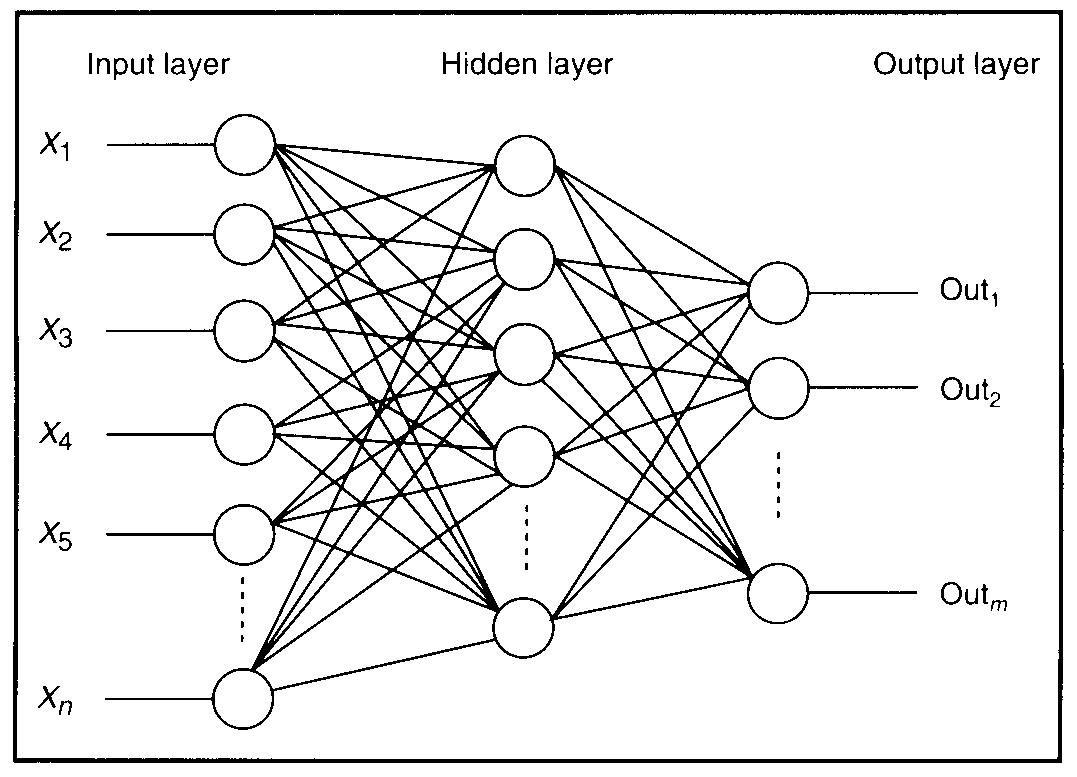
\includegraphics{thesis_figures/NN.jpg}
    \end{center}
    \caption{An example of a Neural Network with two layers -- Source: mechanicalforex.com}
    \label{fig:neural_network}
\end{figure}
% FIXME: figure, check usage rights

The figure~\ref{fig:artificial_neurons} presents the computation involving a particular neuron and its activation.
Let us define the $j$th neuron in the $k$th layer for the inner-product case, then its output $z^k_j$ is defined:
\begin{eqnarray}
    z^k_j = \sum_{i=1}^{U^{k-1}} w^k_{i,j} z^{k-1}_i + b^k_j
\end{eqnarray}
where $U^k$ is the number of neurons in layer $k$.
Then we define the $j$th neuron in the $k$th layer for the activation case:
\begin{eqnarray}
    z^k_j = g(z^{k-1}_j, w^k_{j})
\end{eqnarray}
where $g$ is the activation function with its parameter.
Most of them use the sigmoid activation function and connect each neuron to all the next layer neurons.
Training the weights generally involves gradient descent to minimize the loss function of such networks.
This loss represents the error between the prediction of the network (its output) versus the expected output (in classification: the class label).
The training involves an iterative process where: the input is first feed-forwarded into the network to compute the error, then this latter is back-propagated up to the first layer, while each unit weights is adjusted to minimize the unit error.
This process should be repeated until the error on the validation set has converged to a local optimum.

\begin{figure}[t]
    \begin{center}
        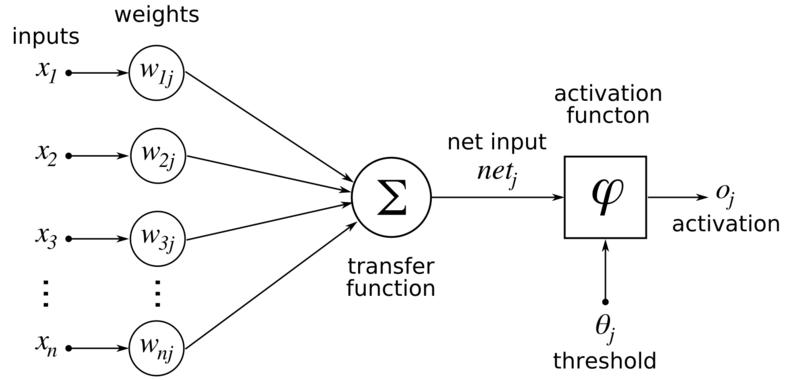
\includegraphics{thesis_figures/800px-ArtificialNeuronModel_english.jpg}
    \end{center}
    \caption{A neuron computing an inner-product with a link to its activation neuron -- Source: Wikipedia}
    \label{fig:artificial_neurons}
\end{figure}

One particular architecture is the CNN, a special case of NN with certain restrictions.
CNN models learn very effective solutions for many Computer Vision problems in image classification.
We briefly describe below three main ideas: local receptive fields, weight sharing and subsampling.
In CNN, a convolutional layer can model receptive fields by computing multiple trainable 2D kernels which is convoluted with its entire input whose result is called its feature maps.
We can see a kernel convolution as the replication of a single unit along the dimensions of the input (a 2D grid for images), thus all weights are constrained to be equal by definition.
A convolutional layer contains multiple units where each has its own kernel.
Therefore different kernels are applied to the image where a single kernel convolution is called a feature map.
Such layer naturally computes filters which can be seen like data-driven feature extractors.
The benefit of weight sharing in convolutional layers is to reduce the number of global parameters to learn general purpose filters which can increase generalization.
Usually, CNNs have subsampling layers right after convolutional layers to reduce the dimensionality of the feature maps so that more concise and high-level information are extracted.
Most CNN architectures puts multiple convolutional layers connected to the input to extract visual features after which they have regular inner-product layers (see figure~\ref{fig:convnet}).
CNN can be seen as two parts: a trainable feature extractor made by the convolutional network followed by a neural network classifier.
Although CNNs have more constraints, it has been shown they generally outperform NN in multiple Computer Vision problems because they learn more invariance\cite{simard2003best}\cite{mnist_web}\cite{lawrence1997face}\cite{krizhevsky2012imagenet}.

\begin{figure}[t]
    \begin{center}
        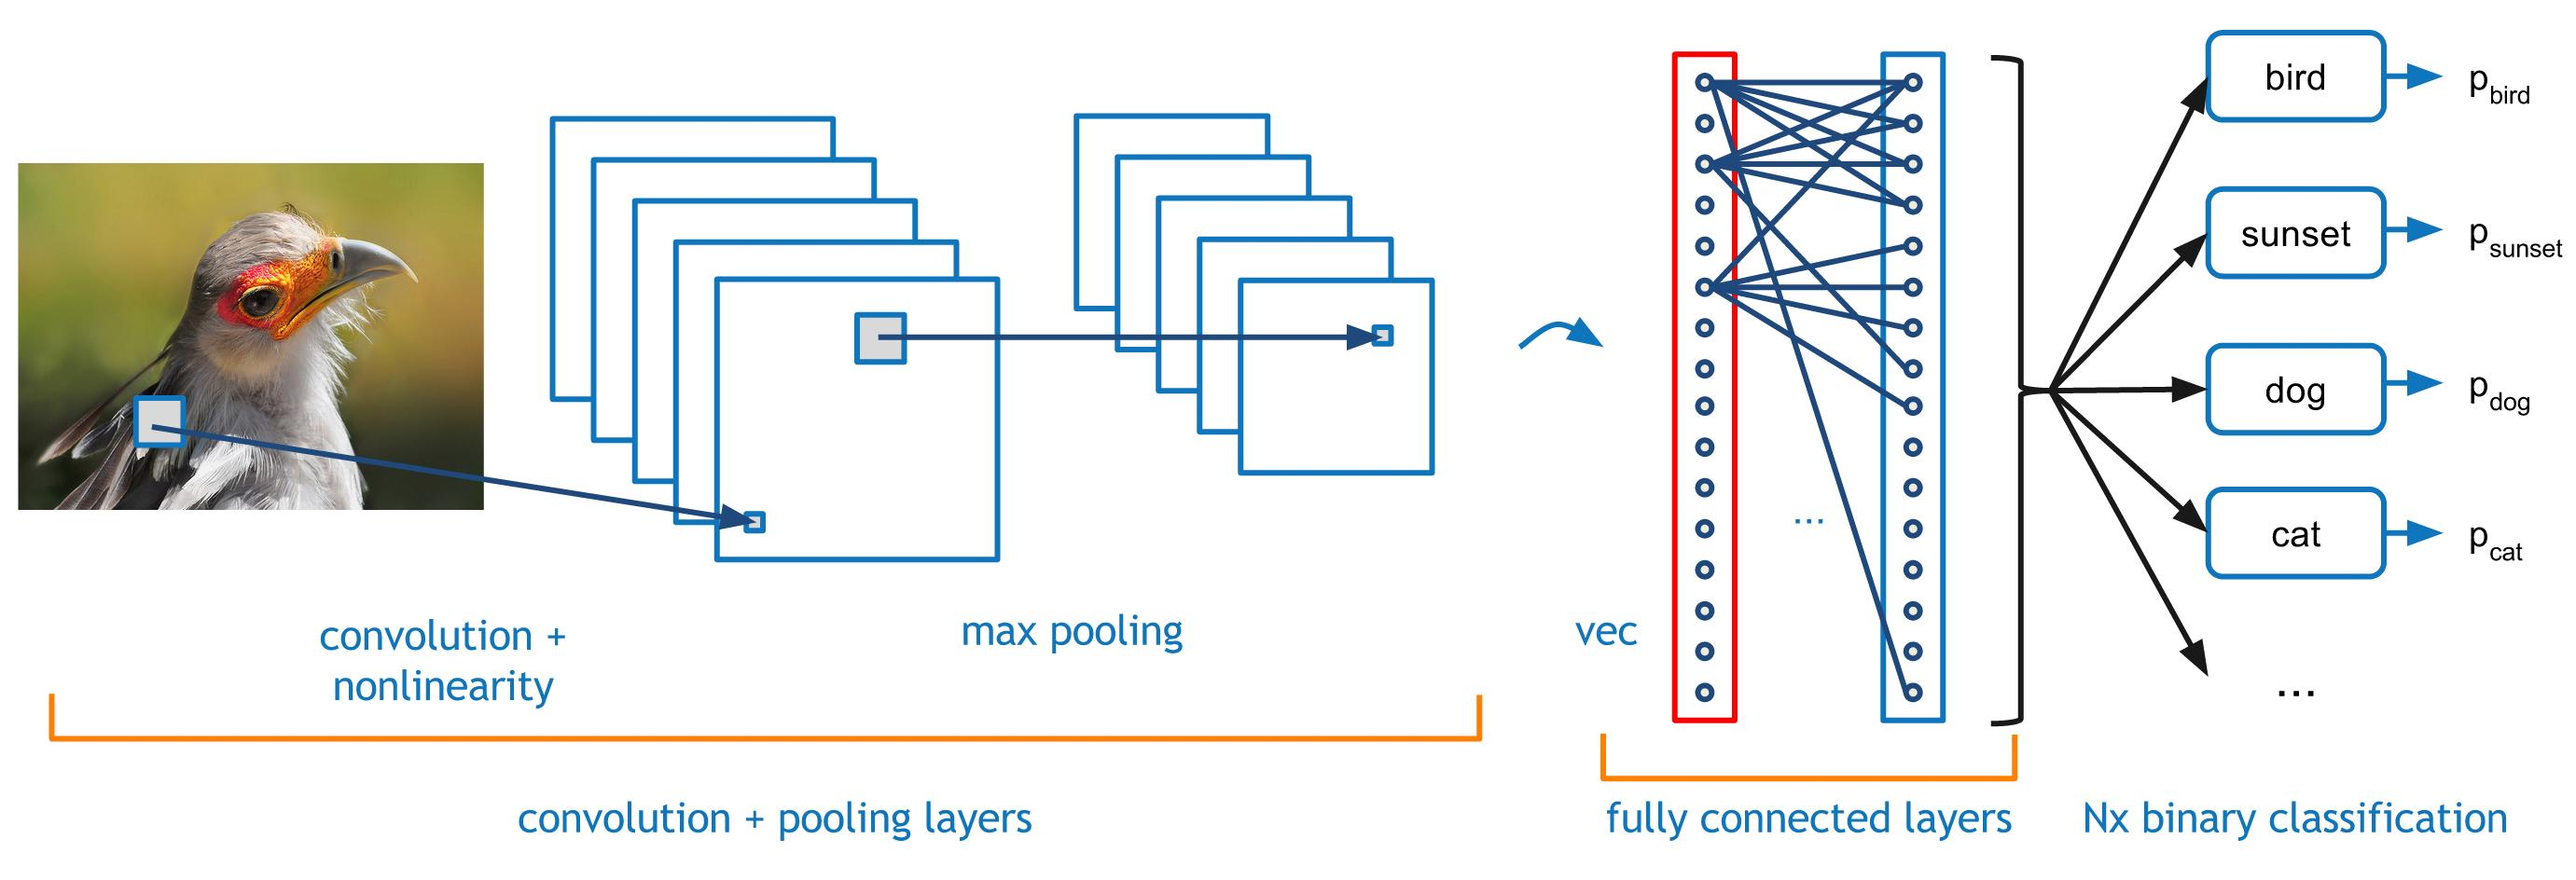
\includegraphics[width=\textwidth]{thesis_figures/conv-net2.jpg}
    \end{center}
    \caption{Architecture of a CNN where the computation flow is explicitly shown -- Source: code.flickr.net}
    \label{fig:convnet}
\end{figure}
% FIXME: figure, check usage rights

Moreover, research found interesting structures in the last-layer embedding of classification NN using t-SNE.
The last layer tends to cluster samples of the same class together while separating the rest\cite{donahue2013decaf}\cite{yu2014visualizing}.
This is explained by the fact that deeper layers extract more high-level information, which is necessary to separate classes. Moreover the prediction is a direct product with the last layer, which encourage the network to have a simple structure directly clustered by classes.
% FIXME: move into dim red chapter?
Thus it is reasonable to evaluate the quality of this embedding as a dimensionality reduction method with great potential to capture more information compared to PCA which captures linear correlations.
It is important to note that t-SNE plays an important role in the quality of this 2D embedding: that is why it can reasonably separates MNIST without any prior treatment.
However, it is important to remember it is not the sole responsible of the better separation using the NN embedding because it has no knowledge of the labels.
The classifier seems to provide better informations to t-SNE which is improving the quality of the structures of the final embedding as we will show later.
%because it learned specialized filters to distinguish the classes.
%Therefore as well as with the help of the classifier features.
This justifies why we combined CNN classifiers with t-SNE to create a 2D embedding for our visualisations.


% ==============================================================================
\chapter{Theory: Dimensionality reduction}
\label{chap:dim_red}
Dimensionality reduction is an important method in machine learning that maps points in a high-dimensional space into a space with a lower number of dimensions.
We will call this lower subspace an {\em embedding}.
Representations suitable for human visualization should keep important relations between points of the original space.
In our experiments, we will apply dimensionality reduction on our neural networks' outputs.
This allows us to quickly compare qualitatively the impact of controlled distortions applied on images over the networks' outputs.
The structure inferred by distances between points such as clusters, intra-cluster neighbors and inter-cluster outsiders reveals important properties of neural network models.
Thus we need accurate low-dimensional representations of embeddings that preserve local distances to compare different models.
In the following sections, we will discuss dimensionality reduction methods that were not fit for our uses, then we introduce in details the one we used, called t-SNE.

\section{Optimisation Problem}
Various algorithms differentiate themselves by several properties: their goal (\eg: interpolation, compression, visualization), by what they preserve (\eg: variance, distances), how they model point correlation (\eg: linearly or not) or whether they can model new points (\eg: a representation or a mapping).

First, our choice is guided by our primary need, which is to visualize our data.
Thus the method should produce a 2D or 3D embedding, preferably in 2D, for easily interpretable scatter plots.
Secondly, we need an optimization problem that keeping certain relations between points such that clusters are equivalently represented.
This can be implemented by preserving relative distances to close neighborhood.
Considering the previous works we discussed above, t-SNE is the best candidate in the current state-of-the-art.
We now define the method objective functions, probabilities and explain intuitive properties.

%introduce theory of SNE, then t-SNE modification.
Let us define our dataset $D$ formed by points in the input-space $X$ of dimension $N$: $D = \left\{ x_1, x_2, \dots, x_n \right\}$, each $x_i \in \R^N$, and one representation $D^\ast$ in the output-space $Y$ of dimension $M$: $D^\ast = \left\{ y_1, y_2, \dots, y_n \right\}$, each $y_i \in \R^M$.
The process of dimensionality reduction is to find the best representation $D^\ast$ that best preserves the most ``important'' information between $x_i$ and $y_i$ for each point.
SNE uses two Gaussian distributions for each point expressing the neighbor distances in $X$ and its equivalent in $Y$.
The Kullback-Leibler divergence is used to compute the objective function, which represents the mismatch of these two distribution for each pair:
\begin{eqnarray}
    L = \sum_{i=1}^n KL(P_i || Q_i) = \sum_{i=1}^n \sum_{j=1}^n p_{j|i} \log\left(\frac{p_{j|i}}{q_{j|i}}\right)
\end{eqnarray}
The probability for a pair of point $x_i$ electing $x_j$ in $X$ follows a Gaussian is as follows:
\begin{eqnarray}
    p_{j|i} = \frac{\exp(-|x_i - x_j|^2 / 2 \sigma_i^2)}{\sum_{k \not = i} \exp(-|x_i - x_k|^2 / 2 \sigma_i^2 )}
    %&
    %q_{j|i} = \frac{\exp(-|y_i - y_j|^2)}{\sum_{k \not = i} \exp(-|y_i - y_k|^2)}
\end{eqnarray}
The equivalent probability $q_{j|i}$ in $Y$ is the same except that $\sigma = 0$ and $x$ is replaced by $y$.
Therefore, a closer pair implies a higher neighbor-election probability because the distance is low.
This cost function gives an asymmetrical importance to the distances: nearby points in $X$ are greatly penalized if they are far in $Y$; whereas a small cost is incurred for pairs far in $X$ but close in $Y$.
%There is a simple physical interpretation of the SNE optimisation problem: pairs are modeled by asymmetrical springs in a mechanical system, the best solution is when the system is still.

As we said SNE suffers from crowdedness problems in the middle of the embedding and the optimisation is harder due to the asymmetrical nature of the objective function.
Both problems were addressed in t-SNE which give very good results in practice.
The two major differences with t-SNE is the symmetrization of the cost function and replaces the distributions of the embedding by student variants.
In t-SNE, a single objective function is minimized:
\begin{eqnarray}
    L = \sum_{i=1}^n KL(P || Q) = \sum_{i=1}^n \sum_{j=1}^n p_{ij} \log\left(\frac{p_{ij}}{q_{ij}}\right)
\end{eqnarray}
where:
\begin{eqnarray}
    p_{ij} = \frac{p_{j|i} + p_{i|j}}{2 n}
\end{eqnarray}
which forces outliers points to contribute more to the loss.
And:
\begin{eqnarray}
    q_{ij} = \frac{1 / (1 + |y_i - y_j|^2)}{\sum_{k \not = l} 1/(1 + |y_k - y_l|^2)}
\end{eqnarray}
which replaces the $q$ distribution in SNE by a Student with a heavier tail: distances in high dimensional spaces spread across more dimensions; in low dimensional space, the accurate equivalent distance needs to be much higher per dimension (thus more points end up further in $Y$, a heavier tail than in $X$).
As before, a point cannot elect itself: $p_{ii} = q_{ii} = 0$ and probabilities are symmetric for both distributions: $p_{ij} = p_{ji}$ and $q_{ij} = q_{ji}$.
As stated previously the input space $X$ has much more dimensions were distances can be expressed than the 2 dimensions of $Y$.
In summary, t-SNE uses Kullback-Leibler divergence to minimize the mismatch of these two spaces by means of probabilities, therefore the chance of important local structures (frequent patterns) being preserved is higher than with other methods (mosts do not express this goal through an objective function).
Global structures is encouraged by the coherence of the local structures as the divergence decreases and the system stabilizes.

\section{CNN for Dimensionality Reduction}
Usual dimensionality reductions like t-SNE are helpful for many visualizing tasks but it has important drawbacks as well.
We think the most important ones are: the computational cost, the incapacity of mapping new points and the indirect control over the resulting embedding.
Current implementations of t-SNE are still rare, unpolished and require tricks to make them tractable in practice (\eg: reducing first with PCA).
Moreover, there is currently no way with t-SNE to map new points (not in $D$) without optimizing the whole system from scratch.
Besides, t-SNE parameters like perplexity and learning rate are not simple to chose.
Fortunately there are new promising alternatives directly harnessing the power of NN.
We introduce such models in the following section.

%there is a direct way to learn an embedding with CNN without t-SNE.
CNN are mostly used for classification but we can optimize them for other purposes as well.
Instead of the SoftMax loss function used for classification, we can use a special training architecture with a suitable loss that when optimized tries to satisfy some constraints.
For example to create an embedding with chosen properties directly found into the output layer.
Moreover the ideas presented by reduction methods like t-SNE can be formulated in different terms to be applicable to NN.
In our case the most important idea is to keep similar points together and dissimilar far away from each other.

The Siamese network combined with a contrastive loss is a good practical solution to train such networks\cite{bromley1993signature}\cite{chopra2005learning}.
Let us define $G_W$, the function that computes the network output, with parameters $W$ (see figure~\ref{fig:siamese_network}).
Then the Siamese network put two weight-sharing instances of $G_W$ side by side, each having their own input.
On top of this Siamese network is placed the ``cost module'', the contrastive loss, which will compute a loss proportional to the difference between the two output.
The complete network takes a pair of images as input, each image fed into a single $G_W$ instance, and the output is computed over their outputs.
The idea is to optimize the metric between points represented by $G_W$ and to spread contributions between the weights because they are shared.
At the end, when the network is used, only a single instance of $G_W$ is required to feed an input and $G_W$ gives the dimensionality-reduced point.

\begin{figure}[t]
    \begin{center}
        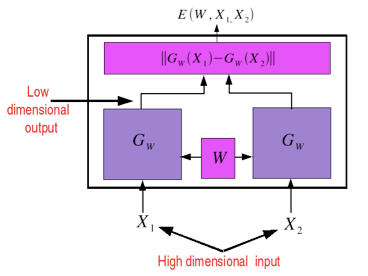
\includegraphics[width=0.5\textwidth]{thesis_figures/siamese_network.jpg}
    \end{center}
    \caption{Schematic representation of a Siamese network -- Source:~\cite{bromley1993signature}}
    \label{fig:siamese_network}
\end{figure}
% FIXME: figure, check usage rights

The contrastive loss function takes its root from Energy-Based Models (figure~\ref{fig:contrastive_spring}).
The loss is constructed as follows.
An attractive term is used to assemble similar points together.
However it would not suffice to make reasonable embeddings because it would allow degenerate solutions where all points squashed together.
To fix this, an opposing term is added to push dissimilar pairs.
Therefore a balance between the two terms is found when the system has converged.

More formally, the definition of the contrastive loss for a pair is as follows:
\begin{eqnarray}
    L = \frac{1}{2} Y (D_W)^2 + \frac{1}{2} (1-Y) \max(0, m - D_W)^2
\end{eqnarray}
where $Y \in \{0,1\}$ is the label: $1$ for similar pairs, $0$ otherwise; $D_W \in \R^N$ is the difference between the two network outputs and the parameter $m \in \R$ defines the minimal distance between dissimilar points.

\begin{figure}[t]
    \begin{center}
        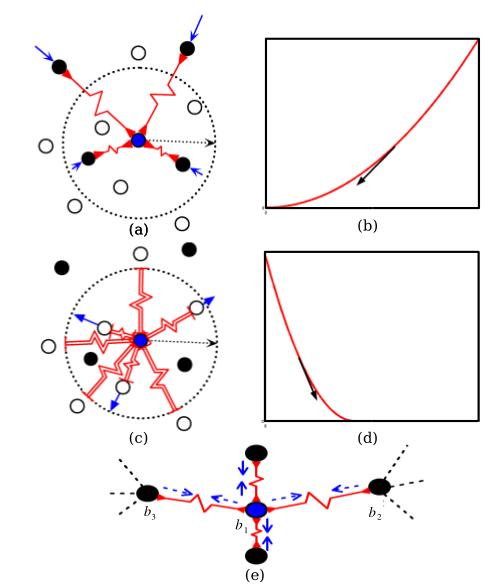
\includegraphics[width=0.5\textwidth]{thesis_figures/contrastive_spring.jpg}
    \end{center}
    \caption{A schematic representation of the contrastive loss using physical springs. Consult \cite{hadsell2006dimensionality} for more details. (a) Shows the points connected to similar points with {\em attract-only} springs. (b) The loss function and its gardient associated with similar pairs. (c) The point connected only with dissimilar points inside the circle of radius $m$ with {\em m-repulse-only} springs. (d) Shows the loss function and its gradient associated with dissimilar pairs. (e) Shows the situation where a point is pulled by other points in different directions, creating equilibrium -- Source \cite{hadsell2006dimensionality}}
    \label{fig:contrastive_spring}
\end{figure}

In the contrastive loss, a label means whether a pair should be close in the embedding but the definition of similarity is left open for the application.

\section{CNN for Predictable Reduction}
The method above can learn an embedding which groups points or separates them based on the pairing strategy but there is still room for improvement.
First, the structure of the resulting embedding is determined by the dataset and again we indirectly shape it by giving a single boolean information per pair which helps to constraint local structures.
However, there is no guarantee that this system will converge to an intended global structure with so many dimensions, such as: the ordering of the deformations (\eg: from lowest to highest) or their distribution (\eg: a line, plane or circle).
Secondly, the training required to make the embedding converge to a desirable structure can happen after a long time, after trying different initialization seeds or can never happen at all, and this is partially due to the lack of constraint in the task.
When the number of embedding dimensions, $M$, is higher than the dimension of the pairing, $1$, the model can become unpredictable because more dimensions give more freedom in the way to represent these pairs arbitrarily.

To improve this situation, we propose to add more constraints on such dimensions directly into the optimisation process.
We propose to give more than one information per pair and that allows to shape and guide the ordering of the embedding directly through the loss function.
Our method allows to control separately the usage of each dimension to express simultaneously different properties of our dataset.
To accomplish that, we generalize the contrastive loss to work on training pairs with $p$-dimensional labels and an embedding with $M$ dimensions, where $p \leq N$ by definition.
In this framework, an embedding dimension is allocated to one particular component of the label and one component can be expressed through one or more embedding dimensions.
The allocation of the embedding dimensions and the pairing strategy are left open to the use-case.

We now introduce our loss function with a formal definition.
Let us define $M$ as the number of embedding dimensions, $p$ the dimensions of the labels and $p \leq M$.
We define $D \in \N_+^p$ as the number of embedding dimensions assigned for each label component.
In this work, we only consider problems where each dimension is assigned to a single label and no dimension is left unconstrained: $\sum_i^p D_i = M$.
Then it follows that the definition of the generalized $p$-dimensional contrastive loss for a pair is:
\begin{eqnarray}
    L = \frac{1}{2} \sum_{i=1}^p \left( Y_i (D_{Wi})^2 + (1-Y_i) \max(0, m_i - D_{Wi})^2 \right)
\end{eqnarray}
where $Y \in \{0,1\}^p$ with $Y_i$ being the $i$th component of $Y$, $D_{Wi} \in \R^{D_i}$ is the difference between the two points in the sub-embedding for dimensions of the $i$th component, and $m_i \in \R$ is the minimal distance for dimension $i$.


% ==============================================================================
\chapter{Methodology and Results}
\label{chap:results}

In this chapter, we will describe the general environment we used to make our experiments, the settings to reproduce them and their outcomes.
We introduce the different models in details with their architecture, then we explain our implementation using Caffe and Python.
We discuss how our datasets are generated by combining samples from MNIST or NORB.
Finally, we present how we will later compute quantitatively measure for comparisons with prior arts.

\section{Models and parameters}

%explain our models.
As previously said, we are closely following the work of our reference paper \cite{hadsell2006dimensionality}.
Therefore, we employ the same two models to experiment on their respective datasets MNIST and NORB.
The first model is {\bf LeNet 5}, a multi-layer neural networks that is characterized by an architecture designed for handwritten characters as illustrated in figure~\ref{fig:siamese_cnn}.
It is with no surprise that they are using it for MNIST, which is the most popular handwritten digit dataset for research.
In our experiments with this dataset, we are using a very close fine-tuned variant with minor changes described below.

\begin{figure}[t]
    \begin{center}
        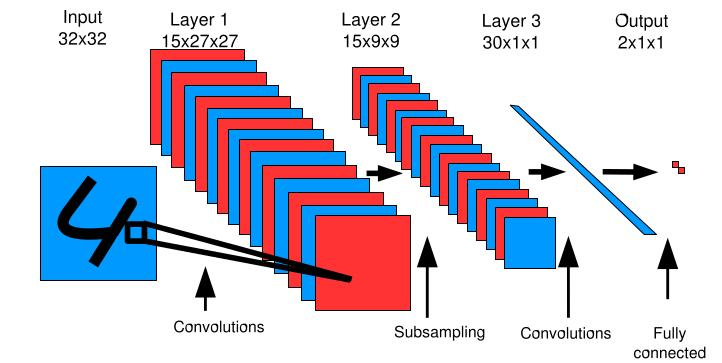
\includegraphics{thesis_figures/siamese_cnn.jpg}
    \end{center}
    \caption{Architecture of the CNN used for our experiments on MNIST (based on LeNet 5). The network contains two convolutions layer which are connected by a subsampling layer and the final output is computed by a fully-connected layer. The computation flow is illustrated for a region of an image. -- Source: \cite{hadsell2006dimensionality}}
    \label{fig:siamese_cnn}
\end{figure}

This network architecture is comprised of a total of 7 layers with trainable parameters.
The first part of this network is comprised of two pairs of convolution-pooling layers, where convolution kernels share their weights.
As explained earlier, each convolution is applied to the entire image to create a single feature map.
The first convolutional layer has 20 different trainable $5 \times 5$ kernels, which is followed by a trainable $2 \times 2$ max-pooling layer (with a stride of $2$).
The second convolutional layer has 50 trainable $5 \times 5$ kernels, followed again by a $2 \times 2$ max-pool layer (stride $2$).
The convolutional network ({\em convnet}) part, made by these two pairs of layers, are {\em feature extractors} for this network, it will extract features related to high-level cues to detect digits (\eg: straight or curved strokes).

The second part of this network is composed of two fully-connected layers where only the first one is followed by a non-linear layer.
The first layer has 500 trainable units computing an inner-product, followed by a non-trainable Rectified Linear Unit (ReLU) activations\cite{nair2010rectified}, followed by 10 trainable output units computing an inner-product which gives the digit class (1 versus rest).

The second model is composed of only two fully-connected inner-product layers.
This network is much simpler than the one above because it is trained on a subset of the NORB dataset, which exhibits very few variability (compared to MNIST).
The two layers are made of 20 and 3 trainable units respectively, without non-linearity between them. % FIXME: non-linearity, really?

In the following experiments, we will train our variant of LeNet in two different ways: for digit classification to analyze the ``natural'' embedding and with a Siamese training architecture with the contrastive loss function to analyze a ``constrained'' embedding.
For our second model, we will only train a ``constrained'' embedding with the Siamese architecture for NORB, like in our reference paper.
It is important to note that in the LeNet ``constrained'' experiment we keep only a single fully-connected layer with the number of trainable units equals to the embedding dimensions (\eg: $2$ or $3$).
The motivation is that the classification task is built on top of the network stack generating this embedding but in our second experiment we need this output rawly, like in our reference paper.

In the case of digit classification, the model is trained using Stochastic Gradient Descend (SGD) with a learning rate of 0.01 optimizing a SoftMax loss function.
Siamese models are trained with SGD with a learning rate between 0.01 and 0.001 optimizing the contrastive loss.

For this project we chose the {\bf Caffe} deep-learning framework to train our models.
There are several reasons among them: the simplicity to express networks, train or manipulate them; Caffe includes several network implementations for MNIST with LeNet and Siamese networks, for ImageNet with AlexNet, GoogLeNet where pre-trained versions are available; Moreover Caffe is well optimized C++ with CUDA GPU parallelism, it is flexible including official Python and MatLab bindings and its community is very active and helpful.

For our experiments on MNIST we could easily adapt the provided LeNet to match the architecture design discussed above.
For the second non-convolutional network, we wrote the network definition ourself due to the triviality of this task.
The training stage need many special parameters related to the solver (SGD): learning rate, batch size, momentum, weight decay (gamma and power) and number of epoch.
They were kept unchanged because the Caffe community already fine-tuned them.
We limited all our experiments to $10'000$ iterations, with a batch size of $64$.
All our networks were trained using the Caffe built-in solver provided with the binary using {\tt caffe train}.
Our alternative loss function was implemented in a new loss layer like the built-in contrastive loss.
Our implementation is straightforward with NumPy in Python and the caffe bindings were used to integrate our layer into the network architecture.

% FIXME: add figures

Most of our experiments were implemented using the Python scripting language: to generate our transformed datasets, to compute quantitative measures and visualization projections.
We created our own set of tools to generate distorted training sets for our t-SNE experiments and to generate the distorted pairs training sets for our two Siamese experiments.
The scikit-learn Python library ({\em sklearn}) now implements most of the standard algorithms for machine learning including the one we used: PCA and t-SNE\cite{pedregosa2011scikit}.
The performance of t-SNE depends heavily on the number of input dimensions and in our experiments we had to apply PCA on our datasets first like other papers suggest\cite{t-SNE} (to compute t-SNE in a reasonable amount of time).
We followed sklearn suggesting to always reduce to $50$ dimensions with PCA before applying t-SNE\footnote{t-SNE documentation page: \url{http://scikit-learn.org/stable/modules/generated/sklearn.manifold.TSNE.html}}.
% FIXME: make source available?

For the visualization of our resulting embeddings, we developed our own solution based on the web library {\em CanvasJS}.
Its main advantage is to allow to interactively visualize with scatter plots directly from the output of t-SNE or the neural networks.
Several features were already provided: coloring points, fast plotting for interactivity; But some were implemented ourself: zooming and moving the viewport, display the image of any sample and filtering/highlighting capabilities to our own application.
All this functionalities give us the necessary tools to inspect qualitatively the results so that at the end we possess the insights we needed.

\subsection{Datasets}
%introduce datasets: mnist and norb.
To perform our experiments, we used two different datasets: {\bf MNIST}\cite{lecun1998mnist} (popular handwritten digit dataset) and {\bf NORB}\cite{lecun2004learning} (popular figures photography dataset).
We briefly present each dataset with some sample images, we give a few insights about their variability and their usual usage in Computer Vision.

The {\bf MNIST} dataset ({\em modified National Institute of Standards and Technology}) is a gathering of multiple databases of handwritten digits.
One of the goal of MNIST is to provide a unified benchmark for digit recognition and it is widely used in Computer Vision for many years.
It is composed of $60'000$ training and $10'000$ testing images of digits between $0$ and $9$.
A few examples of the training set are illustrated in figure~\ref{fig:mnist}.
The samples are heavily post-processed: uniform black background, white-shaded digits with bold strokes.
The digits are centered such that the gravity center is in the middle and size-normalized so one digit lies inside a restrained sub-region of the $28 \times 28$ bitmap.
The variability of this dataset lies in the different strokes, different writer styles, natural rotations, thickness, curve roundedness and such.
The MNIST dataset is considered nowadays extremely simple, like a toy example due to the lack of natural variability and because state-of-the-art achieved extremely good results.
However it is still a good subject of experiments to try and validate new ideas easily as it is in our case.

\begin{figure}[t]
    \begin{center}
        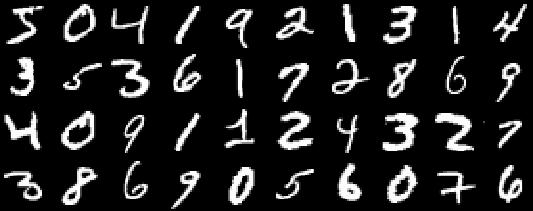
\includegraphics{thesis_figures/mnist.jpg}
    \end{center}
    \caption{A few image samples taken from the MNIST training set to illustrate the dataset. Images were concatenated to save space.}
    \label{fig:mnist}
\end{figure}

The {\bf NORB} dataset ({\em NYU Object Recognition Benchmark}) is a collection of photos of toy figures taken from a variety of contiguous poses.
This dataset has two variants where we picked the normalized-uniform set.
Its usage is also intended for benchmark, in ``large-scale invariant object categorization''.
It is composed of $48'600$ processed photos of toy, see figure~\ref{fig:norb}.
The dataset is made by combining: $9$ elevation views, $18$ azimuth views, $6$ illumination conditions and $5$ toys categories, each containing $10$ toys.
The categories are: humans, animals, airplanes, trucks and cars.
The usual training task is to recognize the toy category whatever viewpoint or illumination is used.
However the reference paper uses only the images of a single plane toy, to infer a representation of the distortions in 3D.
As we are doing comparisons with their methods, we will use the same toy to make our results as well.

\begin{figure}[t]
    \begin{center}
        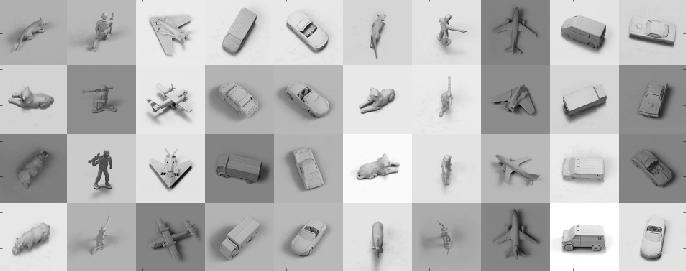
\includegraphics{thesis_figures/norb.jpg}
    \end{center}
    \caption{A few samples taken from the NORB training set to illustrate the dataset. Images were concatenated to save save.}
    \label{fig:norb}
\end{figure}

%how we create our train/test dataset
Our experiments require to process the images in a systematic and coherent way.
We are using Python scripts to automatically derive our training and testing set in a predictable way based on the original dataset (MNIST and NORB).
The training architecture apply sequentially SGD over the samples in batch as they appear and it loops over the whole dataset if the number of iterations has not reached zero.
The generation of our datasets depends on multiple parameters related to the experiment.
In the case of the t-SNE visualization, we create a distorted dataset containing each sample plus its distorted versions varying in strength, where each image has only a single transformation at a time.
The samples are all distorted using the same set of intensities, quantified as follows: translations and shearing using pixel displacement, rotations using positive and negative angles and blurring with averaging radius (examples in figure~\ref{fig:mnist_transfo_tsne}.
In the case of Siamese training, we create paired datasets: containing two distorted images with their similarity (1 or 0).
Images in a pair can have different distortions and different classes (digit for MNIST, elevation/azimuth for NORB) and still be paired (label 1), depending on the experiment.
An example of pairs for MNIST is illustrated in figure~\ref{fig:mnist_pairs}.

\begin{figure}[t]
    \begin{center}
        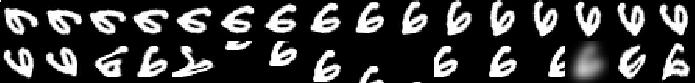
\includegraphics{thesis_figures/mnist_transfo_tsne.jpg}
    \end{center}
    \caption{Illustration of some distortions applied to a random sample included in our data-augmented dataset used in the t-SNE visualization experiment. The following distortions are shown: translations, rotations, blurring and linear deformation}
    \label{fig:mnist_transfo_tsne}
\end{figure}

\begin{figure}[t]
    \begin{center}
        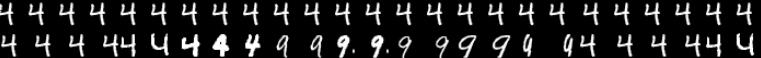
\includegraphics{thesis_figures/mnist_pairs.jpg}
    \end{center}
    \caption{Illustration of some pairs generated for a random sample with its distortions, neighbors and non-neighbors. The pairs are included in our training dataset for our Siamese network.}
    \label{fig:mnist_pairs}
\end{figure}

In the experiments with t-SNE, we are generating a classification task where the training dataset contains one untouched and multiple translated digits with the corresponding label.
This process is called {\em data augmentation}: the dataset is grown artificially by reusing samples but distorted by translations to train invariant models.
Each sample is present with several combinations of increasing translations.
The objective is to train an invariant network and inspect the underlying embedding by using t-SNE.
The goal of this experiments is two folds.
First we would like to understand classifier embeddings and its interaction with t-SNE in a practical manner: testing various data-augmentation methods to see how it impacts the model, its accuracy and how t-SNE adapts.
Secondly, this experiment tests whether we can get an embedding with our prerequisites properties of predictability with a state-of-the-art method specialized for projecting in 2D.

% for siamese
In the Siamese experiments, in order to compare our results to the reference paper, we trained two models based on their settings on MNIST and NORB.
The goal of DrLIM is to train a model where points are close together if they are ``visually'' similar without considering distortions depending on the dataset.
The implementation of their pairing strategy is as follows.
First they group each sample into a common ``neighborhood'' relation the 5 most similar ones using the euclidean distance in pixel space.
However in practice, neighbors with different digit class would appear and DrLIM's paper did not mention if they considered legit or not.
In our case we decided to only consider neighborhood with the same class after a visual inspection (we found such pairs enough dissimilar).
The sample and its $n$ translations are all paired with both its 5 neighbors and all its $n$ translations (this sums up to $n \times 5n$ pairs per sample).
All other pairs are considered dissimilar: when the two samples are not part of the same common translated neighborhood.
This strategy uses the regular contrastive loss function in 1D with a single similarity per pair.

Our objective is similar in the sense that we want to stay invariant but only in certain dimensions of our choice.
Our implementation can still quantify distortions by expression them in the other dimensions.
One important advantage is to allow more control, especially in how dimensions are used.
As we said, we are training a single model which is less expensive and allow to learn reusable features for multiple pairings.
%invariance to distortion but our implementation allow to keep a predictable quantification
We can use our extension of the contrastive loss function with $p$ labels for each pair.
The definitions of $p$ and $D$ for the two Siamese experiments are now described and justified in the following.

In the case of MNIST, we are using a 3-dimensional embedding space: where the first two dimensions express neighborhood similarity and the last dimension expresses the distortion similarity.
It is true 2D suffices in this case but to be comparable to DrLIM's 2D embedding, we will use a 2D neighborhood space as well and separate distortions into its own space.
Making comparisons between 2D space (DrLIM) and 1D neighborhood (our model) would be unfair due to distances increasing very quickly as the number of dimensions increases.
In this settings, we have: $M=3$ (embedding dimensions), $p = 2$ (two labels) and $D = \left\{ 2, 1 \right\}$ (2D + 1D).
We train our network using a similar pair strategy to DrLIM but with important differences.
Our first label considers: a sample and its translations to be similar; the sample and its neighbors to be similar if they have the same translations; and the sample and any non-neighbor sample to be dissimilar with or without translation.
We call this first label: the ``neighborhood'' similarity.
Our second label considers similar: a sample and any other sample with the same translation; and considers dissimilar any pair without the same translation.
We call this second label: the ``transformation'' similarity.
Pairs not mentioned in our descriptions above are not included in our datasets.
Moreover we reduce the size and the time for training by randomly taking a subset of dissimilar pairs to balance the label ratio instead of including all of them.

In the case of NORB, we are using a 3D embedding as well: where the first 2D are used for the cyclic azimuth (horizontal angle of the viewpoint) and the last 1D for the non-cyclic elevation (vertical angle).
DrLIM's work defined similar pairs when the two images are from contiguous elevation or azimuth and we will do the same.
The justification of DrLIM's dimension allocation is as follows.
The azimuth viewpoint is cyclic and the shape to represent such a structure, without overlapping for different values, is an ellipsis which requires at least 2D.
The elevation viewpoint is not cyclic because NORB has only a smaller subset of values, thus only a single dimension is allocated.
In this case we can directly compare DrLIM's embedding and ours as they work on the same problem.
Thus again we have: $M=3$ (embedding dimensions), $p = 2$ (two labels) and $D = \left\{ 2, 1 \right\}$ (2D + 1D).
We train our network based on DrLIM's pairing strategy where we separate the azimuth and elevation into two labels (instead of having them merged).

\section{Evaluation Metrics}
We know qualitative results can provide insights about model behavior or the quality of embeddings but it has drawbacks.
First it requires a human judgement which requires manual efforts, thus it cannot be systematic and automatic.
Secondly the subjective nature of qualitative measures is subject to different interpretation or can be biased towards certain aspect that people value differently.
We think qualitative judgements are unreliable and should not be used alone to asses the work in NN.
However, DrLIM results are lacking objective measures, for example the final loss or any sense of scale of dimensions to relate in the plots nor does it even talk about any kind of measure to quantify the quality.
We think that by lacking any form of measures, DrLIM paper does not promote the continuation of its work because there is no common way to measure ``better''.
Evaluation metrics are very important to permit objective comparisons between several results to see how they perform.

That is why we propose a very simple quantitative measure that allow us to compare DrLIM and our models.
Models are optimized with respect to their loss functions and indeed the loss is an objective measure that can be directly used to compare models on certain conditions.
Given the same loss, if its parameters are the same then it is logically fair to compare them.
It is logically fair to compare models by computing a common loss function, with the same parameters and on the same dataset.
Therefore, we can use the contrastive loss of DrLIM on its test set using the original pairing strategy.
However, DrLIM paper does not provide the margin which is problematic to reproduce their work.
In our case, we are training our own versions of DrLIM and thus we will use a common margin per dataset for the two models.

% FIXME: continue?
%in our case, we compare the quality of digit neighbor clustering.
%we can use DrLIM dataset, recall pairing.
%recall we project our 3D into 2D to compute loss.
%our model not optimizing this directly, disadvantaged.
%goal is to see the cost of keeping translation.

%need an other measure to compare quality for our goal.
%this measure should account for separation and predictability.

%contribution: how we can compute our energy-distance for comparisons.

\section{Results and Discussion}

We conclude this chapter by presenting our results and insights, including the plots and quantitative measures.
Our first experiment is the visualization of the LeNet embedding on the MNIST classification task.
We compare the structural differences between models trained with and without data-augmentation.
However the resulting embedding has an unexpected structures that does not fit our requirements.
Then, we move on with results of directly optimized embedding with models using the contrastive loss.
We apply DrLIM's methods by replicating the experiments on MNIST and NORB.
Followed by a throughout detailed discussion of our methods in the same conditions to compare the two.

%tables and graphs: loss of training (for major models), add accuracy for comparison, compare DrLIM with ours (energy-distance).

\subsection{t-SNE on LeNet}
%show t-sne on raw mnist to compare?

To create our model, we train on the MNIST classification task to classify digits without any modification.
At this point, all images of the training set are used as is without data-augmentation, thus there is little invariance.
The error rate of this model is 1.0\% which is computed over the MNIST test set.
According to the published results on the MNIST website, this is the expected value (LeNet-5: 0.95)\cite{mnist_web}.
In the following experiments, we consider this network with the classification layers removed (SoftMax and 10-outputs inner-product).
Therefore the last remaining layer is a ReLU which follows the last inner-product of 500 dimensions.
Our hypothesis at this stage is as follows: This last layer should express high-level concepts of digits and we call it the fingerprint.
To understand the behavior of the system, we also include a few distorted samples to the test set: for each digit we select five samples and include their distortions as described in the methodology.
To confirm our intuition, we forward this test set into this network, apply PCA on its output which is given to t-SNE to create the final embedding.
The whole process takes around 45 minutes on a single core.
The resulting embedding is illustrated in the figure~\ref{fig:mnist_nda_tsne} which does not include the distorted samples whereas~\ref{fig:mnist_nda_tsne2} does.
We can see qualitatively on figure~\ref{fig:mnist_nda_tsne} that most of the original digits are well separated where each cluster represents a single class.
The major exception are the 1s spreading on a thin vertical curve over a small part of he 6s.
Our hypothesis seems validated by the structure on this plot: separation of classes and coherence inside clusters by visual inspection.
Most of the distorted samples on figure~\ref{fig:mnist_nda_tsne2} are part of their respective clusters however they drift apart and extremes are outside.
% FIXME: need description of how they drift wrt distortion?

\begin{figure}[t]
    \centering
    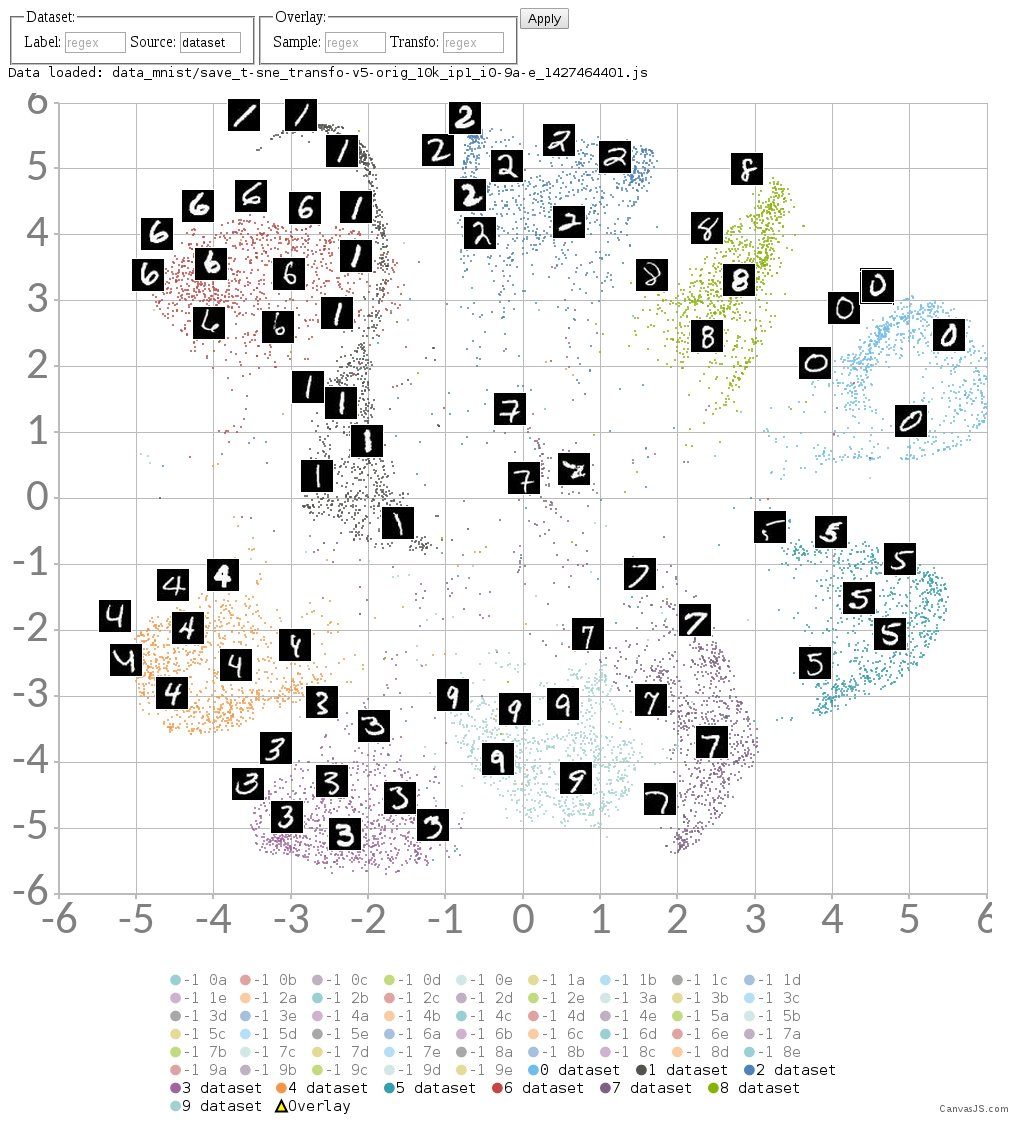
\includegraphics[width=\textwidth]{thesis_figures/mnist_nda_tsne.jpg}
    \caption{Scatter plot of the t-SNE representation of the CNN embedding fed with the MNIST test set using our interactive tool. General view where the distorted samples are hidden. Some random samples are shown for each cluster. Each color represent a digit class.}
    \label{fig:mnist_nda_tsne}
\end{figure}

\begin{figure}[t]
    \centering
    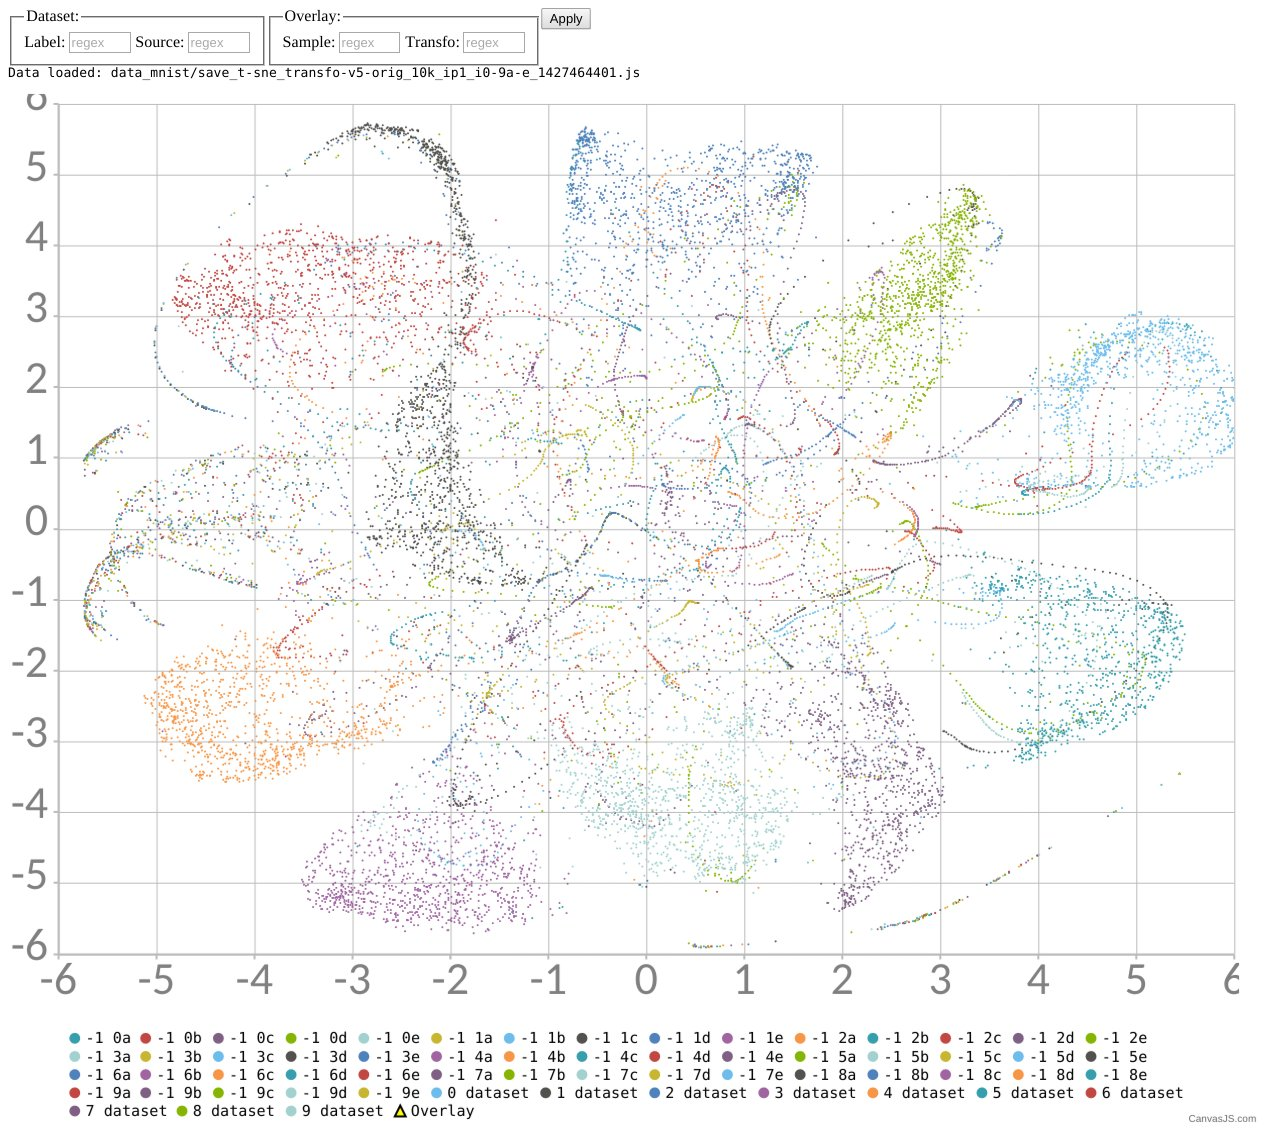
\includegraphics[width=\textwidth]{thesis_figures/mnist_nda_tsne2.jpg}
    \caption{Scatter plot of the t-SNE representation of the CNN embedding fed with the MNIST test set using our interactive tool. Close view of the 0s cluster containing distorted samples. Most of the samples are continuous distortions of the sample sample (same color). A unique color is given to each digit class as before plus one unique color for each sample's distortions.}
    \label{fig:mnist_nda_tsne2}
\end{figure}[t]

In the next experiment, we apply the same process with a translation-invariant model.
One simple way to achieve invariance is to train the model over a data-augmented training set to distinguish centred digits as well as translated digits.
As previously described, our augmentation consists of a range of translations applied to all samples which are included into the training set.
In our case we chose all translations in $x$ between $-5$ to $+5$ plus translations in $y$ between $-10$ and $+10$.
The error rate on the original test set increased up to $3.5\%$, but we do not have comparisons for this value.
However this model has a strong translation invariance because its error rate is only $8.5\%$ on the data-augmented test set (we must stress the fact that it contains extreme translations).
Our second hypothesis is as follows: As the fingerprint contains many different features, it should also detect translations which was heavily present in the training set.
We can now compare the embeddings of this new model (see figure~\ref{fig:mnist_da_tsne}) versus the one above.
From a general perspective, translations are dominating the global structure of the clusters.
The centered digits are still in their own clusters but most of the translated ones are grouped disregarding their class.
However the ``translated'' clusters exhibits coherence: sub-clusters represent digit classes but they are heavily overlapping.
For example, the right-displaced digits are exclusively appearing in the top-left corner where all digits are present and mostly stacked together in the center.
This is actually a general problem with this plot: many clusters appear but their delimitations are fuzzy which suggests it would be hard to quantify translations and digits.

\begin{figure}[t]
    \begin{center}
        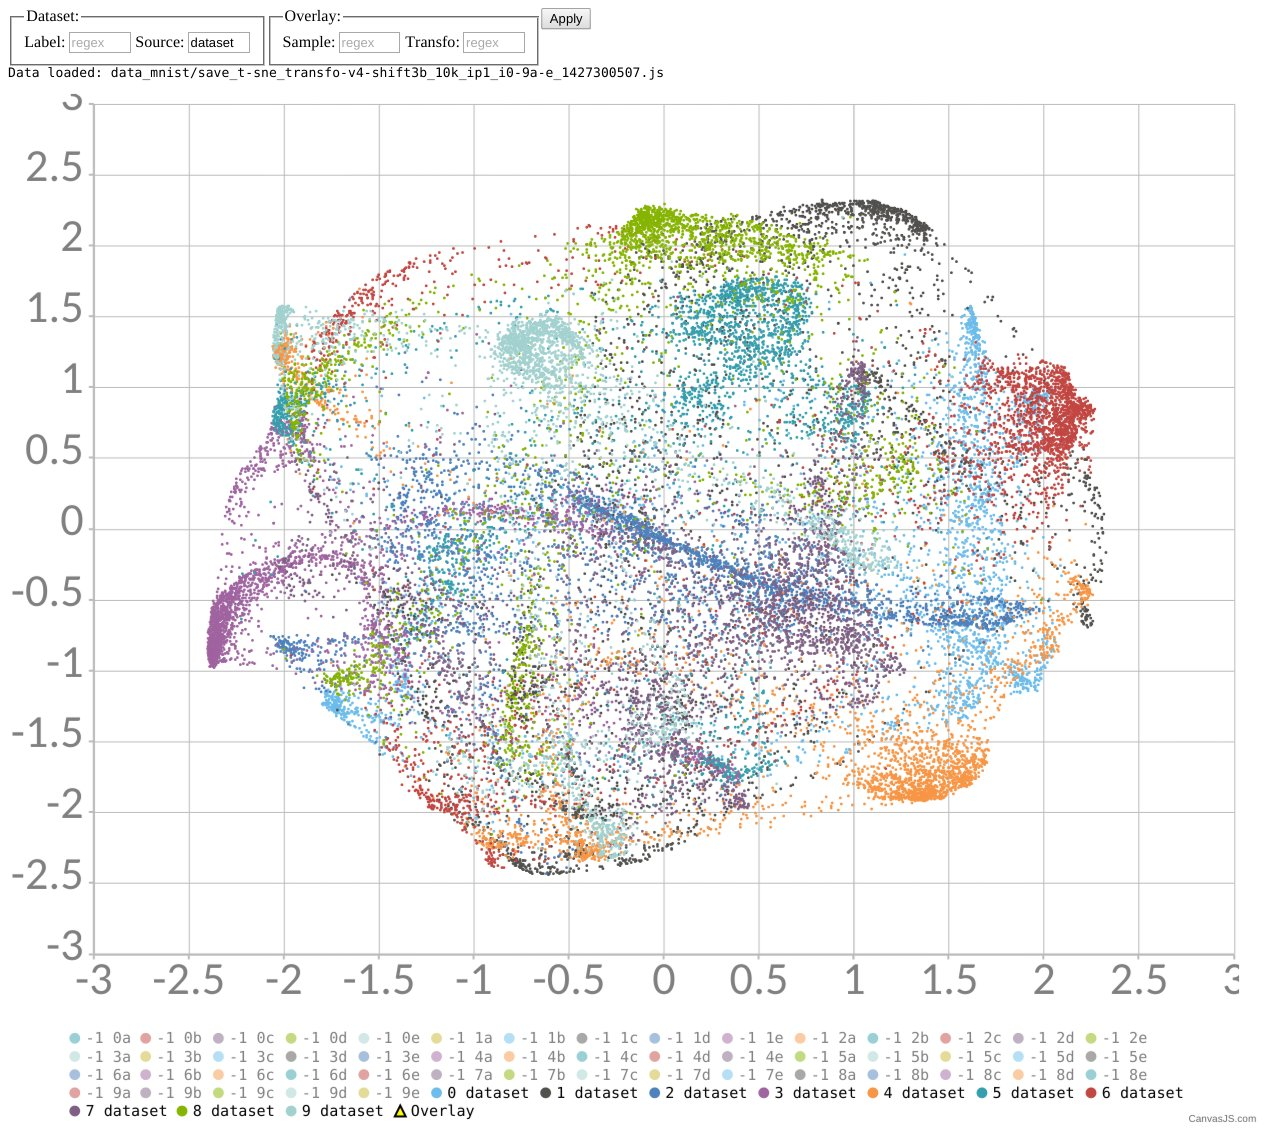
\includegraphics[width=\textwidth]{thesis_figures/mnist_da_tsne.jpg}
    \end{center}
    \caption{Scatter plot of t-SNE representation of the CNN embedding fed with the data-augmented MNIST test set using our interactive tool. A unique color is attributed to each digit class and one for each sample's distortions as before. The digits shown were manually selected to represent the local trend.}
    \label{fig:mnist_da_tsne}
\end{figure}

%discussion.
%give insights: about t-sne, models, clustering, etc.
From these two experiments, we learn important knowledge about NN on simple classification tasks, about data-augmentation and t-SNE as well.
Manual experiments confirmed that LeNet is sensitive to the distortions we used and can easily misclassify if no form data-augmentation is used during training.
As we said, nearly no natural distortion is left in the dataset and this is mostly due to the heavy prior processing applied to the MNIST dataset
However small rotations are still present in MNIST which explains why our model is less prone to errors on artificially rotated samples.
Data-augmentation is an effective way to reduce the error rate on certain type of distortions but it has a cost.
In our case t-SNE embedding looks ``overcrowded'' and most cluster are not well separated anymore.
We think it is due to the important difference of energy in the pixel space, \eg: the center of mass is translated.
One explanation is that the network learned to separate this source of variance and acquired position-specific features to distinguish translated digits which impacts fingerprints of the last layer.
Then t-SNE is impacted by clustering translations first, then digits as its second major structure.
One important insight is that t-SNE represents hierarchical structures with decreasing importance due to its optimization formulation thus the most discriminative features would be weighted more.
% FIXME: check this claim

We consider these results unexpected: the clusters are not well separated and they are lacking in coherence even though the task require to separate the digits.
This experiment is meant to create an invariant model for classification but the representation of the fingerprint does not naturally split digits and translations into different axes.
We have to repeat again that t-SNE is oriented towards visualization whose goal is not formally and universally well defined.
The current formulation of this method is to preserve distances between the fingerprints of our models which is not sufficient for our application.
There is currently no way to add prior information like supervised methods to guide the optimization to associate particular dimensions to particular variance in the data.
A possible solution is to modify the objective function of t-SNE to reach our goal but it has the important limitations we discussed in the methodology.
The lack of end-to-end optimization in this method is also important and this can be solved by using layers handling the dimensionality reducing into a single NN.

We present, in the following part, results of our alternative method based on end-to-end and supervised training of a single CNN.

\subsection{Contrastive LeNet (MNIST)}

In the two experiments below, we train Siamese networks with the contrastive loss function.
To compare with our reference results, we train for each one a network in the original configurations of DrLIM and an other network with the extension as described in the methodology section for two-label pairs.

The first dataset is a subset of MNIST containing only 4s and 9s digits which we derive our training and testing set based on our 2D pairing strategy.
Therefore the resulting dataset is composed of each sample plus its translations (±3, ±6 pixels) which is then paired.
The models are trained until the loss on the respective test set has attained a reasonable local minima, which takes around 10 minutes.
After around $100$ iterations, both models have reasonably converged to a stable solution (see figure~\ref{fig:mnist_cl2d_loss}).
However, our model has reached a lower solution than DrLIM: comparing them directly is not possible because the two datasets are different but the difference in the loss in our model is more important and converge as quickly.
Intuitively this means that our problem formulation is easier to solve and the model finds a ``better'' solution, in the sense it could satisfy more our constraints described by the loss.
The resulting embedding are shown in figures:~\ref{fig:mnist_cl_drlim} for DrLIM and~\ref{fig:mnist_cl2d} for our model.
The DrLIM embedding we reproduced is very similar to the excepted result: a coherent grouping based on translation-agnostic similarity; however the separation between digits is more pronounced.
We can look at the DrLIM embedding as a top-down projection of our 3D embedding where the additional vertical dimension quantify the displacement.
The different intensity of translations are well separated into their own cluster as demonstrated by a meticulous manual inspection and remarkably they are ordered vertically by their intensity.
Once again, the space inside clusters is well organized by digit features like DrLIM.

\begin{figure*}[h]
    \centering
    \begin{subfigure}{0.45\textwidth}
        \centering
        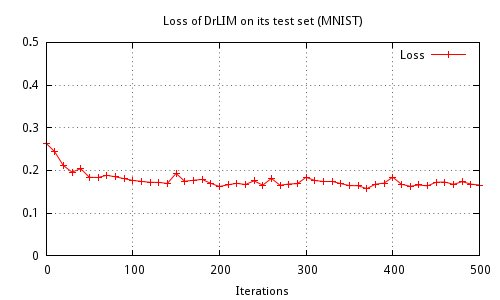
\includegraphics[width=\textwidth]{thesis_figures/final_loss_testset_2bv7.jpg}
        %\caption{Loss of DrLIM}
    \end{subfigure}
    \begin{subfigure}{0.45\textwidth}
        \centering
        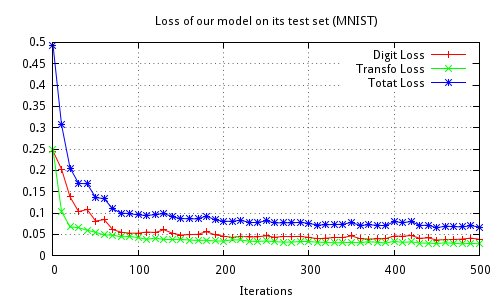
\includegraphics[width=\textwidth]{thesis_figures/final_loss_testset_3Dc3.jpg}
        %\caption{Loss of our model}
    \end{subfigure}
    \caption{Plot of the model loss for 500 iterations of DrLIM and our model on MNIST.}
    \label{fig:mnist_cl2d_loss}
\end{figure*}

In order to compare the two methods, we present quantitative measures where the contrastive loss is computed on the DrLIM paired test set as described in the methodology.
Evolutions of this measure during training are plotted in figure~\ref{fig:loss_mnist_test_common} and the final losses after 10'000 iterations are: $0.160023$ (DrLIM) and 0.145418 (our model).
The two loss series shown in this figure are statistically indistinguishable according to a t-test with a null hypothesis of $\alpha = 0.05$.
Therefore we can conclude our model learns an equivalent representation in its 2D digit-projection to DrLIM with a slightly different formulation and it can expresses distortions without loosing information in its 3rd dimension at the same time.

\begin{figure}[h]
    \centering
    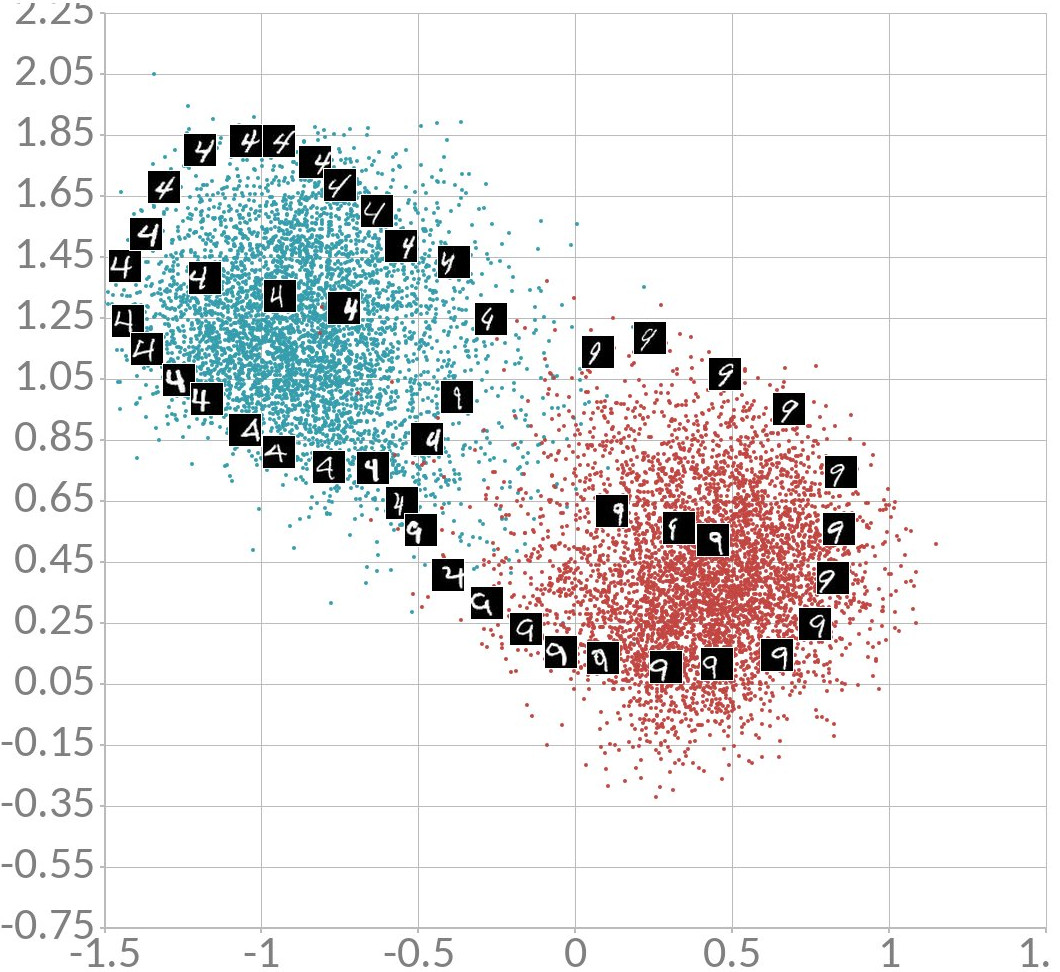
\includegraphics{thesis_figures/mnist_cl_drlim.jpg}
    \caption{Plot of the DrLIM embedding on the MNIST translation-augmented test set where some random samples are shown for illustration.}
    \label{fig:mnist_cl_drlim}
\end{figure}

\begin{figure*}[h]
    \centering
    \begin{subfigure}{0.7\textwidth}
        \centering
        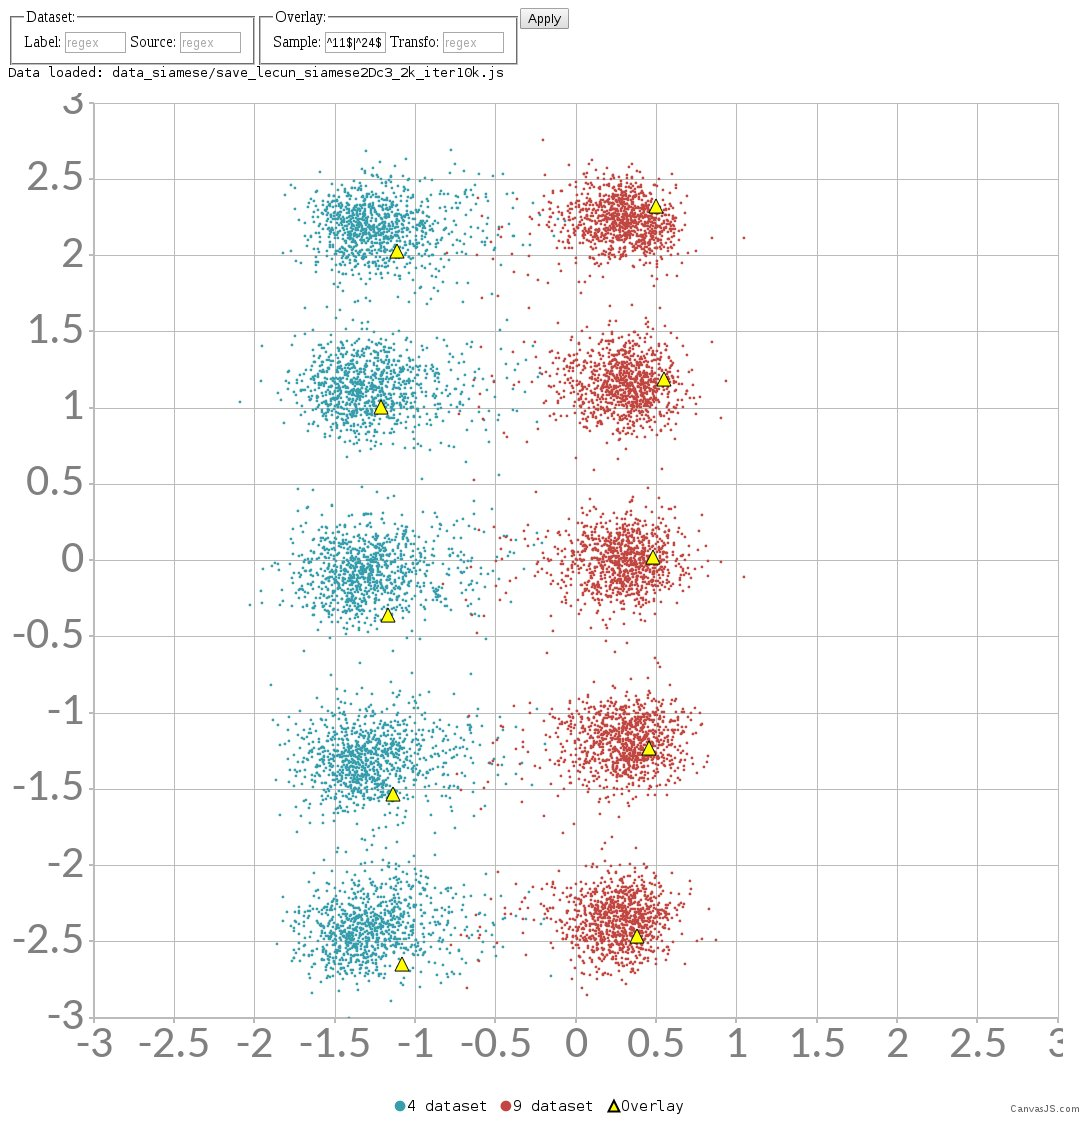
\includegraphics{thesis_figures/mnist_cl2d.jpg}
        \caption{Two samples of different class were selected at random and their distortions are marked as triangles in the figure.}
    \end{subfigure}
    \begin{subfigure}{0.7\textwidth}
        \centering
        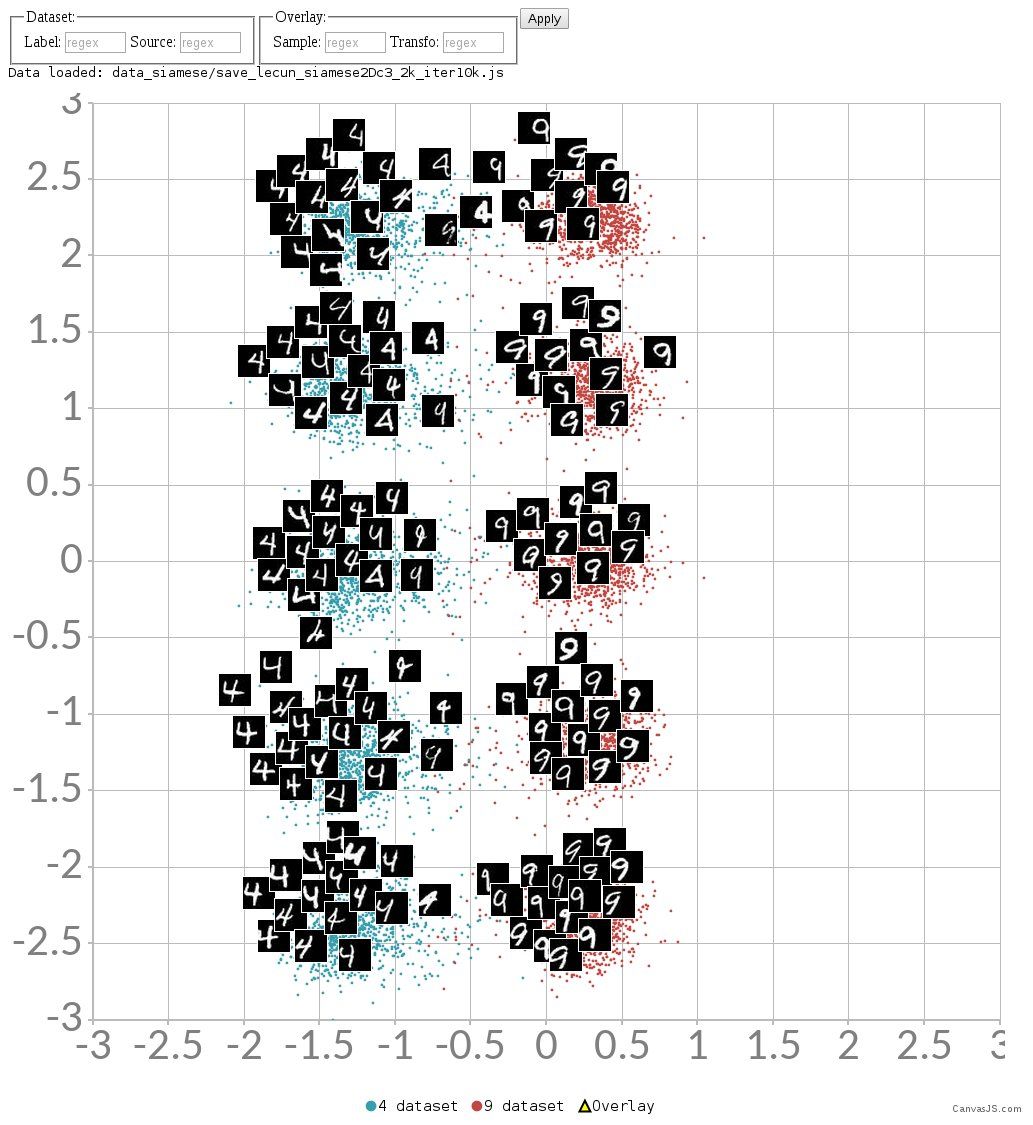
\includegraphics{thesis_figures/mnist_cl2d2.jpg}
        \caption{General view where random sample's distortions are displayed to represent the local trend.}
    \end{subfigure}
    \caption{Plots of our model embedding on the MNIST translation-augmented test set projected in 2D.}
    \label{fig:mnist_cl2d}
\end{figure*}

\begin{figure}[h]
    \begin{center}
        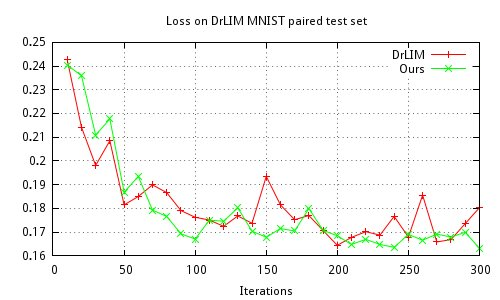
\includegraphics{thesis_figures/final_loss_test2bv7.jpg}
    \end{center}
    \caption{Comparison of quantitative measures between DrLIM and our model during training iterations on the translation-augmented MNIST test set.}
    \label{fig:loss_mnist_test_common}
\end{figure}

We tested our model on a data-augmentation of MNIST based on rotations as well to show it works on non-linear deformations as well.
Clusters are still arranged in a linear fashion although rotations are non-linear but the cluster separations are smaller, see figure~\ref{fig:mnist_cl2d_rotate}.
The results are similar to our previous experiment and we only provide the figure for demonstration as we won't discuss it in more details.

\begin{figure}[h]
    \begin{center}
        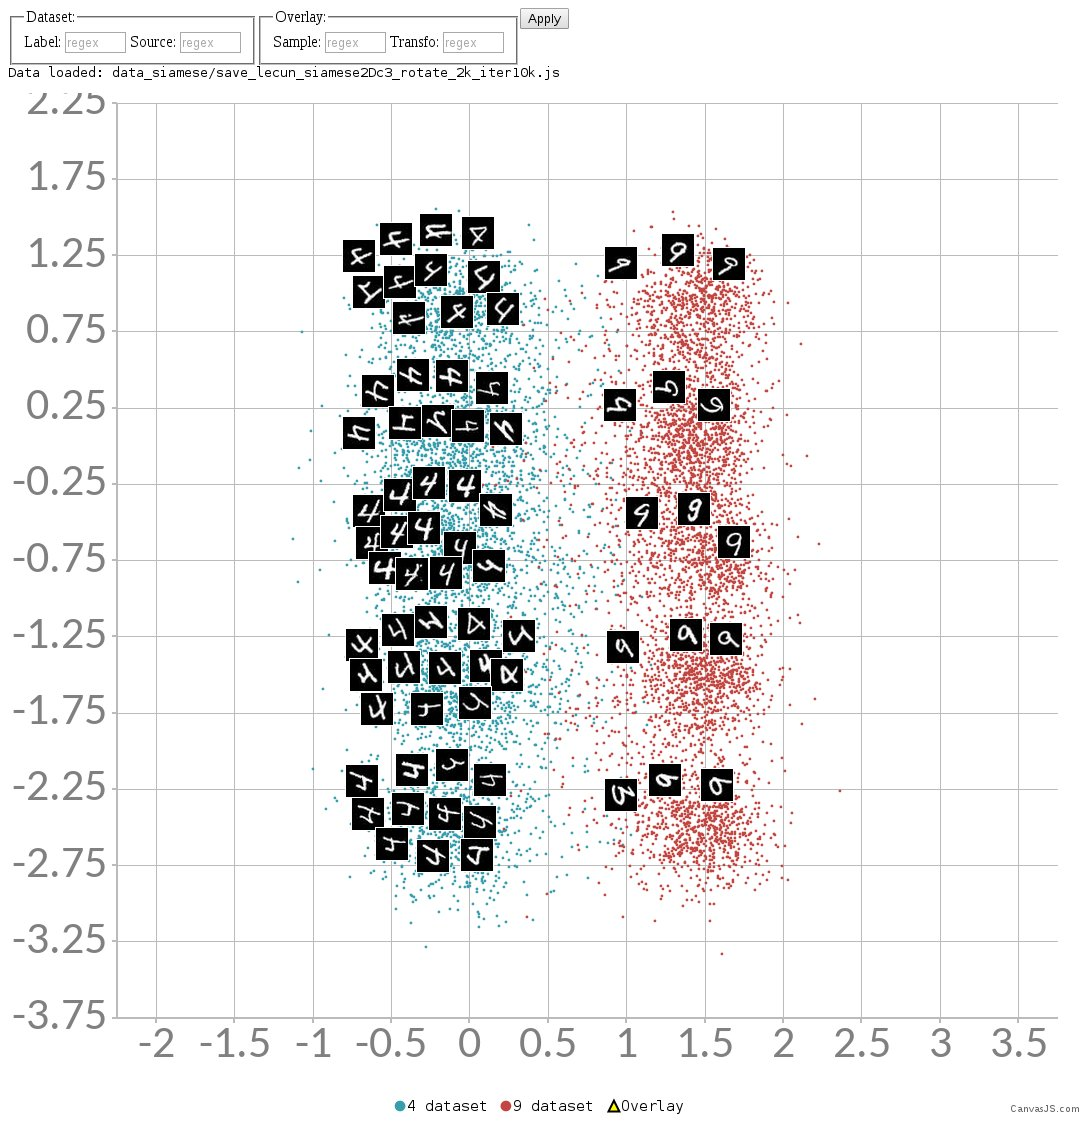
\includegraphics{thesis_figures/mnist_cl2d_rotate.jpg}
    \end{center}
    \caption{Scatter plot of our model embedding on the MNIST rotation-augmented test set}
    \label{fig:mnist_cl2d_rotate}
\end{figure}

\subsection{Contrastive LeNet (NORB)}
Once again we train our network following our conventions, this time on a subset of the NORB dataset with a single plane.
As we previously described, this subset is composed of all viewpoint of a single plane which we call thereafter the 1-plane NORB dataset.
We split this subset into two parts: 660 training samples and 312 test samples.
These two sets are both separately paired according to the strategy described in the methodology to form the training and testing sets.
The models are trained until the loss on the respective test set has attained a reasonable local minima, which takes around 10 minutes.
After $2'000$ iterations, both models have reasonably converged to a stable solution (see figure~\ref{fig:norb_cl2d_loss}).
To get the most convincing results, we had to chose $m=1$ for DrLIM and $m=10$ for our model, therefore their loss on the test set should not be compared directly, instead the quantitative measures below should be used instead.
However we can see DrLIM in figure \ref{fig:norb_drlim_embedding} has an easier formulation this time (smaller margin) and the embedding is very similar to the one presented on DrLIM paper.
The most important features of the embedding to represent NORB is: the cyclic structures for the azimuth angle, the continuity along the two axes disregarding lighting illumination and the sharp separation along the axes.
Indeed, this embedding is a thin cylinder whose long axis represent the elevation and the radius is the azimuth angle.
However, the cylinder is not perfect: multiples parts are more flat along the elevation axis (like a plane) and the radius is fuzzier than presented in the reference paper.
The major difference with our solution, as shown in figure \ref{fig:norb_cl2d_embedding}, is the alignment along the plot axes, a more stable radius and a better separation inside the cylinder.
The predictability of our solution is improved by these properties compared to DrLIM.

\begin{figure*}[h]
    \centering
    \begin{subfigure}{0.45\textwidth}
        \centering
        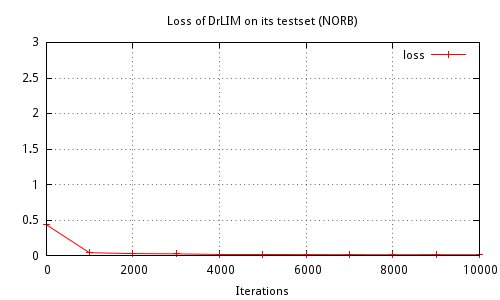
\includegraphics[width=\textwidth]{thesis_figures/final_loss_testset_3d.jpg}
        %\caption{Loss of DrLIM}
    \end{subfigure}
    \begin{subfigure}{0.45\textwidth}
        \centering
        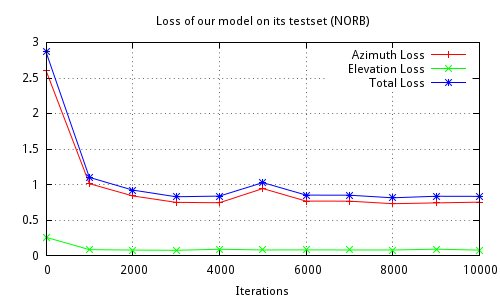
\includegraphics[width=\textwidth]{thesis_figures/final_loss_testset_2D1g2.jpg}
        %\caption{Loss of our model}
    \end{subfigure}
    \caption{Plot of the model loss for 10'000 iterations of DrLIM and our model on NORB.}
    \label{fig:norb_cl2d_loss}
\end{figure*}

\begin{figure*}[h]
    \centering
    \begin{subfigure}{0.45\textwidth}
        \centering
        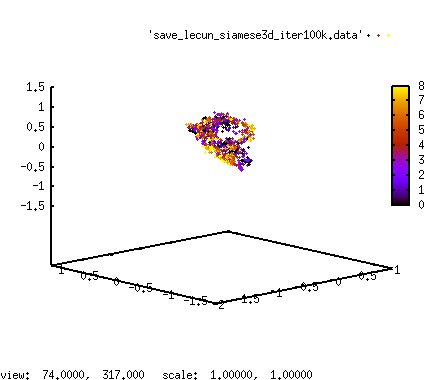
\includegraphics[width=\textwidth]{thesis_figures/norb_drlim1.jpg}
    \end{subfigure}
    \begin{subfigure}{0.45\textwidth}
        \centering
        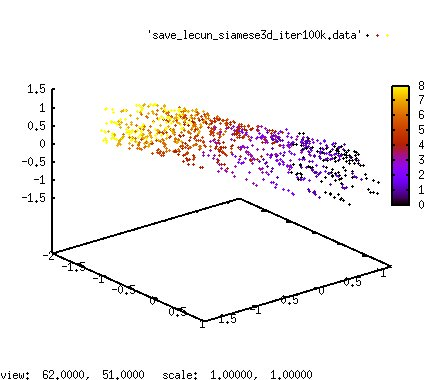
\includegraphics[width=\textwidth]{thesis_figures/norb_drlim2.jpg}
    \end{subfigure}
    \caption{3D Plot of the DrLIM embedding on the NORB 1-plane train+test dataset after $100'000$ iterations. The colors indicate the elevation angle.}
    \label{fig:norb_drlim_embedding}
\end{figure*}

\begin{figure*}[h]
    \centering
    \begin{subfigure}{0.45\textwidth}
        \centering
        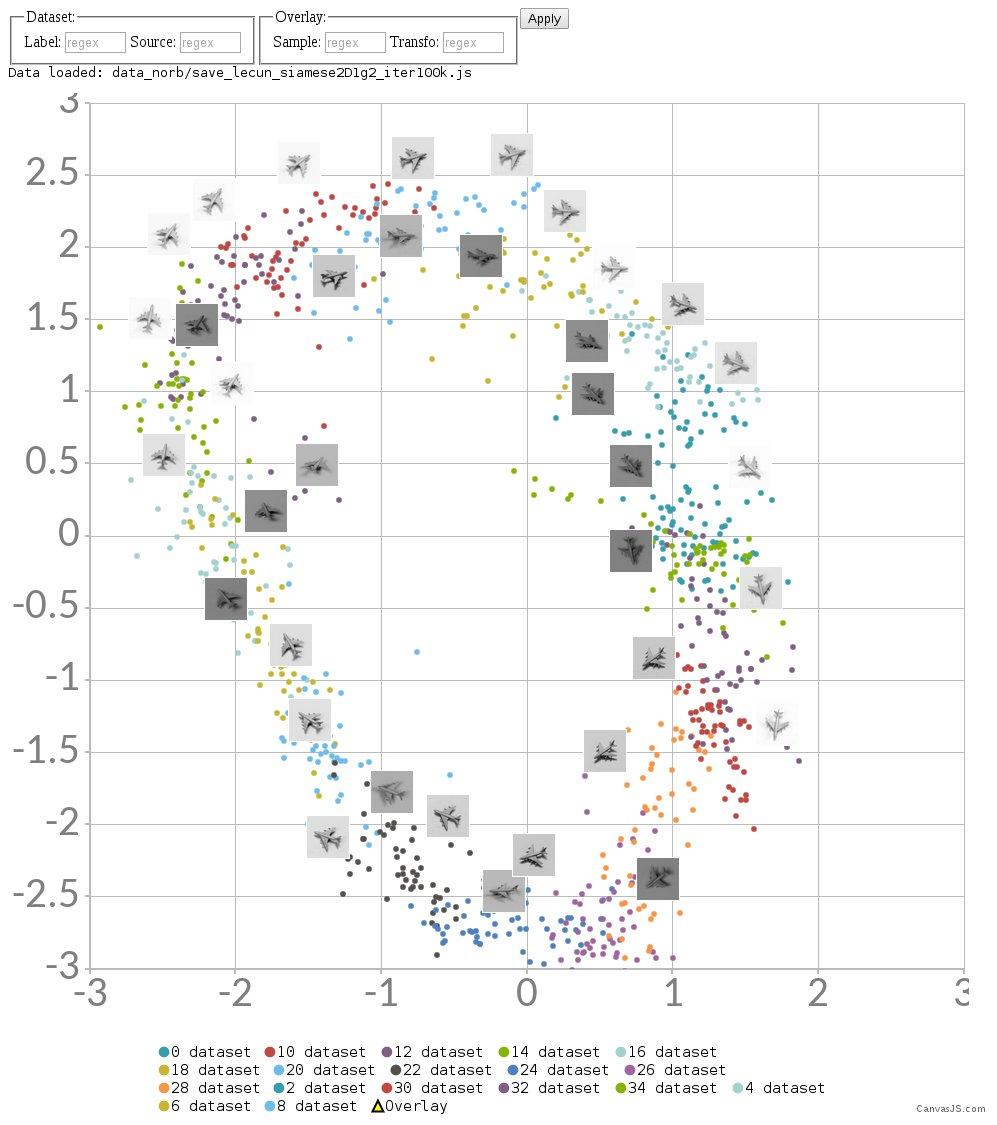
\includegraphics[width=\textwidth]{thesis_figures/norb_cl2d.jpg}
        \caption{2D projection of the first two axes. Colors indicate the azimuth angle.}
    \end{subfigure}
    \begin{subfigure}{0.45\textwidth}
        \centering
        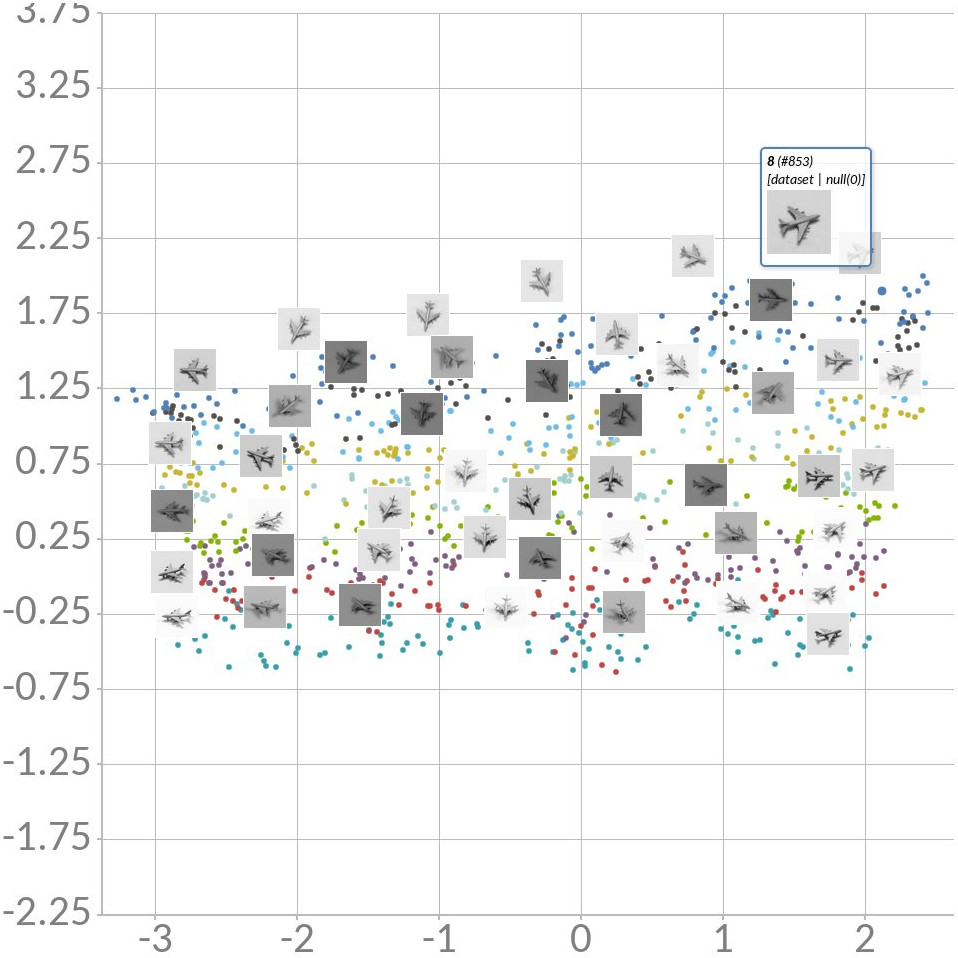
\includegraphics[width=\textwidth]{thesis_figures/norb_cl2d2.jpg}
        \caption{2D projection of the last two axes. Colors indicate the elevation angle.}
    \end{subfigure}
    \caption{2D Plot of our model embedding on the NORB 1-plane train+test after $100'000$ iterations.}
    \label{fig:norb_cl2d_embedding}
\end{figure*}

To compare the two models, we computed the contrastive loss on the test set of the 1-plane NORB with the same parameters ($m=1$) as with MNIST.
The plot of this loss is shown in figure \ref{fig:loss_norb_test_common} where we also added a version of our model with $m=1$.
The embedding of this new model has many aspects of our other model and the main difference is instead of having a round shape for the azimuth, it is similar to a heart which is also cyclic but less desirable in our opinion.
We can see a major difference with our model $m=10$ compared to both DrLIM and our second model $m=1$.
By definition of the loss function, the model is not penalized to put dissimilar pairs further than the margin, therefore it means our model $m=10$ has decided it is better to put similar neighbors further than the other two models.
Moreover, the loss suggests that our model $m=1$ is better but we find qualitatively that our second model is better, although it has a higher loss.
Unfortunately, the visual quality is not reflected by the loss function in this case.

\begin{figure}[h]
    \begin{center}
        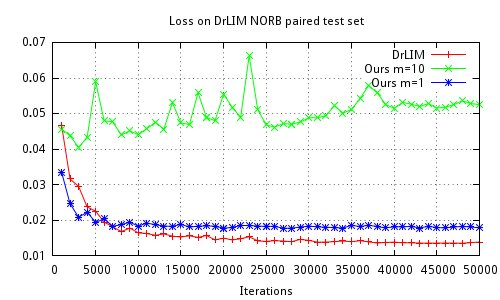
\includegraphics{thesis_figures/final_loss_testv3.jpg}
    \end{center}
    \caption{Comparison of quantitative measures between DrLIM and our model during training iterations on the 1-plane NORB test set.}
    \label{fig:loss_norb_test_common}
\end{figure}

To conclude this chapter, we would like to state a few remarks and overview some difficulties in our experiments.
The primary goal of our experiments using contrastive losses is to show we can expect more predictability in the sense of constraints over the axes, the shape and clusters with a simple extension of the original formulation.
Our qualitative judgement is positive about the success of our experiments.
We demonstrated in our first experiment that models based on DrLIM can include more informations concerning the distortions with minor impact over the original dimensions.
We also demonstrated in our second experiment that they can be guided with minimal efforts to represent the NORB space by using dimensions in a certain way.
Moreover we had great difficulties to reproduce DrLIM on MNIST and especially NORB due to the lack of directives for parameters and due to the initial randomness of model initialization.
During these experiments, we also learned that one if not the most important factor for training a Siamese network comes from the pairing method.
On this regard, many minor factors can greatly impact the final results such as: the ratio of similar/dissimilar pairs, their ordering (shuffled or not) and the addition/removal of certain pairs.
We found our models easier to train because they converged to the above results with nearly no effort: the default weights and margin were safely used and our models converged to the expected solutions.

However there is still room for improvements, especially for the quantitative measures which does not always reflect the structure quality quantified by a visual inspection.
It is important to keep in mind that the visual quality is not necessarily representative of its real usability as features for further layers in a NN.
Nonetheless, it shows that our model can create quite interesting and human-friendly representation by simple methods.


% ==============================================================================
\chapter{Conclusion}
\label{chap:conclusion}

Neural Networks are widely used in many applications of Computer Vision and their usage is growing every day.
The recent usage of NN in dimensionality reduction is an important step to create better embeddings.
Indeed they learn powerful mappings whose relation seems more deeply tied to the dataset: invariance to non-linear distortions and sensibility to certain complex properties unique to the dataset.
In our experiments, we have found NN to be much faster and reliable than even the state-of-the-art methods such as t-SNE where the only cost is some prior-knowledge such as labels or viewpoint angles.
Moreover, many state-of-the-art tricks developed during years of researches on NN have helped us in this task: CNN architecture for images, Siamese network and the contrastive loss function to train our specialized networks.
Thanks to this architecture findings and the current advance in Deep Learning, we benefit from their improvement in the automatic derivation of better features to represent the data.

In this thesis, we showed how t-SNE performs with data-augmentation with its advantages and shortcomings due to its unsupervised nature.
We moved to solutions based on NN because they have many advantages, for example that they can represent very complex mappings.
To achieve a more predictable embedding, we introduced an extension to the previous work on the matter with DrLIM.
Then we experimented with several NN models on different datasets to compare with the state-of-the-art and we demonstrated the effectiveness of our solution.
We presented our qualitative results with figures which we analyzed to understand our models.
But we also introduced quantitative measures based on the loss function to compare more objectively past results with our own.
As we said, there is still room for improvements in this regard as current measures does not seem completely reliable to measure the quality.
Moreover, we tried to develop a better solution which would give a better score not only to compare distances but the predictability of our models.
This solution is non-trivial to find and this would require comparing our models with a simple baseline which does not seem to exist at this day.

The current direction of dimensionality reduction started with DrLIM looks very similar to regression problems and this is also the case for our generalization for N-dimensions.
However regression is more constrained than the current formulation because: (1) clusters can be moved around, only their relative positions matter where their regression counterpart would be forced set at absolute positions (2) the margin formulation allows to put extra gap to make space for clusters without cost whereas regression penalizes in every directions.
Thus, the current formulation allow more freedom in placement than regression which suggests that regression would perform worse due to the addition these artificial constraints.
Future work could compare our models with regression models to see if further restriction would actually help instead.

An other aspect that future research is to test practically the predictability of our embeddings.
For instance by using the produced features in a bigger classification network, for MNIST: gives the distortion intensity and the digit class; for NORB: the two azimuth-elevation angles.
An other useful contribution would find a measure that quantifies the ``predictability'' of our model for certain application.
One simple example would be to use the accuracy of the classification model above but it would not represent the effective usability in practical applications which combine both distortions and application-specific features.
A better example would be a simple model that is trained to derive all distorted inputs' features from one input and the accuracy of such a model would serve as a score.

% applications?
% FIXME: usecase of predictable disto?

% FIXME: to check:
A possible application of our system is in Biomedical Imaging.
Some particular classification tasks in this field (\eg: segmentation) need to detect orientation-dependent structures in images.
The classification of such images begins by a normalization step with a rotation and a translation to normalize the structure of interest into a centered slice
This slice is used to extract orientation-dependant features which are then fed into classifier like a CNN.
It is important to understand the normalization step to extract features like the rotation is costly especially for 3D images where specialized FPGAs are designed only to compute 3D expensive rotations.
Our contribution allows theoretically to bypass this normalization step to directly create the features.
In this case, the model would learn features predictable with respect to the input distortions (\eg: rotations) which means that the features for other distortions can be derived and classified.

In this work we proposed the basic framework to create distortion-predictable models and now practical experiments should be made to show the benefit of our method in similar applications.

%We present a step towards solving this problem efficiently by training a network that quantifies the distortions and exhibits more predictable features under distortions.
%When our model is given a distorted input image, it returns distortion-dependant features and the necessary information to quantify the distortions.
%With such a model it becomes theoretically possible to compute the features of any distortion based on a single pass.
%The derived features can then be fed into very thin orientation-dependant networks to classify structures.

% FIXME: more future works?

% bibliography
\bibliography{thesis}{}
\bibliographystyle{plain}

% required by NORB dataset
\nocite{lecun2004learning}

\end{document}
